% Use the basic LaTeX article class, 12pt text
\documentclass[12pt]{article}

% Science uses Times font. If you don't have this installed (most LaTeX installations will be
% fine) or prefer the old Computer Modern fonts, comment out the following line
% \usepackage{newtxtext,newtxmath}
% Depending on your LaTeX fonts installation, you might get better results with one or both of these:
%\usepackage{mathptmx}
%\usepackage{txfonts}

% Allow external graphics files
\usepackage{graphicx}

% Use US letter sized paper with 1 inch margins
\usepackage[letterpaper,margin=1in]{geometry}

% Double line spacing, including in captions
\linespread{1.5} % For some reason double spacing is 1.5, not 2.0!

% One space after each sentence
\frenchspacing

% Abstract formatting and spacing - no heading
\renewenvironment{abstract}
	{\quotation}
	{\endquotation}

% No date in the title section
\date{}

% Reference section heading
\renewcommand\refname{References and Notes}

% Figure and Table labels in bold
\makeatletter
\renewcommand{\fnum@figure}{\textbf{Figure \thefigure}}
\renewcommand{\fnum@table}{\textbf{Table \thetable}}
\makeatother

% Call the accompanying scicite.sty package.
% This formats citation numbers in Science style.
\usepackage{scicite}

% Provides the \url command, and fixes a crash if URLs or DOIs contain underscores
\usepackage{url}

%%%%%%%%%%%% CUSTOM COMMANDS AND PACKAGES %%%%%%%%%%%%

\usepackage{geometry}
\usepackage{authblk}
\usepackage{booktabs}
\usepackage{tabularx}
\usepackage{amssymb}
\usepackage{setspace}
\usepackage[hypertexnames=false]{hyperref}


\graphicspath{{../figures}}

% Authors can define simple custom commands e.g. as shortcuts to save on typing
% Use \newcommand (not \def) to avoid overwriting existing commands.
% Keep them as simple as possible and note the warning in the text below.
% Example:
\newcommand{\pcc}{\,cm$^{-3}$}	% per cm-cubed

% Please DO NOT import additional external packages or .sty files.
% Those are unlikely to work with our conversion software and will cause problems later.
% Don't add any more \usepackage{} commands.


%%%%%%%%%%%%%%%% TITLE AND AUTHORS %%%%%%%%%%%%%%%%

% Title of the paper.
% Keep it short and understandable by any reader of Science.
% Avoid acronyms or jargon. Use sentence case.
\def\scititle{
A Pandemic-Scale Ancestral Recombination Graph for SARS-CoV-2
}
% Store the title in a variable for reuse in the supplement (otherwise \maketitle deletes it)
\title{\bfseries \boldmath \scititle}

% Author and institution list.
% Institution numbers etc. should be hard-coded, do *not* use the \footnote command.
% \author{
% 	% You can write out first names or use initials - either way is acceptable, but be consistent
% 	First~Author$^{1\ast\dagger}$,
% 	A.~Scientist$^{2\dagger}$,
% 	Someone~E.~Else$^{2}$\and
% 	% Additional lines of authors should be inserted using the \and command (not \\)
% 	% Institution list, in a slightly smaller font
% 	\small$^{1}$Department, Institution, City \& Postal Code, Country.\and
% 	\small$^{2}$Another Department, Different Institution, City \& Postal Code, Country.\and
% 	% Identify at least one corresponding author, with contact email address
% 	\small$^\ast$Corresponding author. Email: example@mail.com\and
% 	% Joint contributions can be indicated like this
% 	\small$^\dagger$These authors contributed equally to this work.
% }

\author[1,2,$\ast$]{Shing~H.~Zhan}
\author[1,$\dagger$]{Yan~Wong}
\author[3,$\dagger$]{Anastasia~Ignatieva}
\author[4]{Katherine~Eaton}
\author[1]{Isobel~Guthrie}
\author[1]{Benjamin~Jeffery}
\author[1,3,5]{Duncan~S.~Palmer}
\author[4]{Carmen~Lia~Murall}
\author[6]{Sarah~P.~Otto}
\author[1]{Jerome~Kelleher}

% %%%  Institutional affiliations should contain the
% %%%  following information at minimum: department(s)/
% %%%  subunit(s), institution, city, state/region (if
% %%%  applicable), and country.

\affil[1]{\small{Big Data Institute, Li Ka Shing Centre for Health
Information and Discovery, University of Oxford, United Kingdom}}
\affil[2]{\small{Infectious Disease Epidemiology Unit (IDEU), Nuffield
Department of Population Health, University of Oxford, Oxford, United Kingdom}}
\affil[3]{\small{Department of Statistics, University of Oxford, United
Kingdom}}
\affil[4]{\small{National Microbiology Laboratory, Public Health Agency of
Canada, Canada}}
\affil[5]{\small{The Pioneer Centre for SMARTbiomed, Big Data Institute, Li Ka
Shing Centre for Health Information and Discovery, University of Oxford, United
Kingdom}}
\affil[6]{\small{Department of Zoology and Biodiversity Research Centre,
University of British Columbia, Vancouver BC Canada}}
% 	\small$^\ast$Corresponding author. Email: example@mail.com\and
% 	% Joint contributions can be indicated like this
% 	\small$^\dagger$These authors contributed equally to this work.
\affil[$\ast$]{\small{Corresponding author: shing.zhan@ndph.ox.ac.uk}}
\affil[$\dagger$]{\small{Joint second author}}

\begin{document}

\maketitle

% Abstract, in bold
% There are strict length limits, and not all formats have abstracts.
% Consult the journal instructions to authors for details.
% Do not cite any references in the abstract.
\begin{abstract}\bfseries
Millions of SARS-CoV-2 genome sequences were collected 
during the COVID-19 pandemic, forming a dataset of unprecedented richness.
Estimated genealogies are fundamental to
understanding this ocean of data 
and form the primary input to many downstream analyses.
A basic assumption of methods to infer genealogies from viral 
genetic data is that recombination is negligible and 
the genealogy is a tree.
However, recombinant lineages have risen to global prevalence, 
and simple tree representations are therefore 
incomplete and potentially misleading.
We present sc2ts, a method to infer reticulate genealogies 
as an Ancestral Recombination Graph (ARG) in real time at pandemic scale.
We infer an ARG for 2.48 million SARS-CoV-2 genomes, 
which leverages the widely used tskit software ecosystem to support further analyses and 
visualisation.
This rich and validated resource clarifies
the relationships among recombinant lineages,
quantifies the rate of recombination over time,
and provides a 
lower bound on detectable recombination.
\end{abstract}

% \section*{KEYWORDS}

% Ancestral recombination graphs, recombination, SARS-CoV-2, ARG, tskit

% SHZ: The first paragraph should explain
% why recombination "can" be important in pathogens.
% Then, we explain why we need recombination-aware methods for pathogens.
% This should set the stage for why this work is really important,
% not just for SC2 but more broadly for the field of pathogen genomics.

% Classical phylo methods fundamentally do not apply to SARS-CoV-2 data, both
% in terms of the basic goal, assumptions about samples and how recombination
% can be treated.
 
% The first paragraph of any Science paper does NOT have a heading
% Nor is it indented
\noindent
Classical phylogenetics is largely concerned with inferring the evolutionary history 
of divergent species~\cite{Felsenstein2004}. 
Recombination among lineages, however, distorts the inference of species trees~\cite{Posada2002effect},
 biases downstream
analyses~\cite{Schierup2000consequences,Hedge2014bacterial}, 
and so requires careful consideration~\cite{Rannala2025recombination}.
Modern pathogen datasets are not sparsely sampled from different species
and may contain millions of genomes sampled from 
% JK: deleted point about recomb here as TB, eg, doesn't
a single species~\cite{
Shu2017,% GISAID ~270k FLU + others
Jolley2018open,% PubMLST, 34K genomes for e.g. Staph Auerus
Apetrei2021hiv,% HIV 1,026,217 sequences
Cryptic2022data,% TB 12k
Dyer2025enterobase% 1 million, various things like E-coli
}.
In contrast to the sophisticated model-based approaches
used to infer species trees~\cite{Suchard2018bayesian,Bouckaert2019beast,Minh2020iq},
comprehensive phylogenies of pathogen datasets are typically built with
simpler distance methods % citation for this?
or approximations~\cite{Price2009fasttree},
primarily due to computational scaling limitations.
While several methods have been proposed to incorporate
recombination explicitly into model-based phylogenetic
inference~\cite{Didelot2010inference,%
Vaughan2017inferring,%
Muller2020bayesian,%
Guo2022recombination,
Muller2022bayesian},
scalability
is a major issue and practical application has been limited.
Software support that explicitly \emph{uses}
recombination-aware inference is mostly restricted to
visualisation, for example of small-scale phylogenetic
networks~\cite{Huson2012,Vaughan2017,Solis-Lemus2017}
or tree changes along the genome~\cite{Rasmussen2023}.

The global
surveillance data collected during the COVID-19 pandemic
presents fundamental challenges to existing approaches. 
First, the sheer amount of data 
overwhelmed even approximate distance matrix-based methods.
% Accessed GISAID/EpiCov on 08 Oct., 2025
At the peak in February 2022, $\sim$80,000 samples per day
were submitted to GISAID~\cite{Shu2017},
accumulating to a total of over 17.5 million samples
as of October 2025.
Regularly re-inferring trees de novo from such rapidly
growing datasets is untenable.
The UShER\cite{Turakhia2021} method is based on adding
samples to an existing tree using maximum parsimony,
with periodic rearrangements to counter the inherent 
greediness of the approach\cite{DeMaio2023}.
The benefits of this simple model and the value of
a comprehensive genealogy updated in real time~\cite{McBroome2021,Kramer2023}
were conclusively demonstrated, as the resource
quickly became an indispensable element
of the pandemic response\cite{Hinrichs2024}.
Recurrent recombination has posed an additional challenge to reconstructing the evolutionary history of
SARS-CoV-2 \cite{Jackson2021,VanInsberghe2021,Focosi2022,
Gutierrez2022,Ignatieva2022,Tamura2023},
with multiple deep recombination events impacting both the genealogy and disease attributes of the virus \cite{Roemer2023,Shiraz2023enhanced}.
Although several methods have been proposed to \emph{detect}
recombinant samples~\cite{Varabyou2021rapid,%Bolotie
Turakhia2022,%RIPPLES
Zhou2023virusrecom,
Alfonsi2024,%RecombinHunt 
Li2024CovRecomb},
this information is not incorporated into the phylogenies used 
in innumerable studies~\cite{McBroome2021,Hadfield2018},
and recombination continues to be treated in a post hoc manner, after phylogenetic reconstruction. 

Ancestral recombination graphs (ARGs) describe the reticulate 
genealogies of sampled sequences in a recombining species\cite{Wong2024},
and provide a natural and efficient means of 
systematically incorporating recombination 
into the study of SARS-CoV-2.
While ARGs have been of theoretical interest in population genetics 
for several decades\cite{Hudson1983,Griffiths1991two,Griffiths1997ancestral},
recent breakthroughs in
simulation\cite{Kelleher2016,Kelleher2018efficient,Haller2019,Gopalan2025bridging}
and inference~\cite{Rasmussen2014,Speidel2019,Kelleher2019,
Wohns2022,Zhang2023,Gunnarsson2024,Deng2025robust} have led to a surge 
of interest in their application in population and statistical 
genetics\cite{Brandt2024,Lewanski2024,Nielsen2025}.
% This is necessary because a bunch of the phylo literature refers
% to ARGs, but it's all in the "coalescent with recombination" sense
% Rannala2025 dismisses ARG-based methods at a stroke because they're
% all based on the assumption of a single panmictic population 
As the range of applications for ARGs has broadened, the term has itself evolved from a specific model of coalescence with 
recombination  \cite{Hudson1983,Griffiths1997ancestral}to a rich data structure representing recombinant ancestry\cite{Minichiello2006mapping,Wong2024}.
The development of extensive software support has facilitated the broader application of ARGS. In particular, the collaboratively built tskit library~\cite{Ralph2020} underpins a 
rapidly growing software ecosystem of
simulation~\cite{Baumdicker2022,Haller2019,Petr2023,Tsambos2023link,Tagami2024tstrait},
visualisation~\cite{Karthikeyan2025tsbrowse,Kitchens2025tskit,Talbot2025argscape},
inference~\cite{Kelleher2019,Wohns2022,Mahmoudi2022,Martin2025model,Pieszko2025detecting}
% More here? I'm sure there's others
and data analysis~\cite{Fan2022,Nowbandegani2023extremely,Fritze2024forest}
tools.

Here we present sc2ts, a new method to infer ARGs for SARS-CoV-2  
that sequentially adds samples over time in a similar manner 
to UShER, while automatically detecting and incorporating recombination
in real-time. Based on the freely-available Viridian dataset, a curated
% NOTE: Viridian doesn't provide alignments, we do that with MAFFT
collection of SARS-CoV-2 genomes purged of various systematic errors and artifacts~\cite{Hunt2024},
we infer an ARG with 2.48 million whole genome sequences.
We show that the non-recombinant portions of this ARG are congruent with the UShER phylogeny built 
from the same dataset as well as the Pango nomenclature system~\cite{Rambaut2020}.
The ARG also accurately captures evolutionary features such as mutational 
spectra~\cite{Bloom2023} and deletions\cite{Li2023indels}.
We show that sc2ts automatically and accurately detects details about
known recombinant lineages that were painstakingly collated through a community effort and provides novel insights into the relationships between these
recombinant lineages. We compare the recombination events detected by 
sc2ts with the state-of-the-art combination of UShER and 
RIPPLES~\cite{Turakhia2022}, showing that sc2ts is more sensitive,
detecting more of the well-characterised recombination events 
curated by the Pango lineage designation community.
The output of sc2ts---incorporating
genealogical relationships, point mutations, deletions, and 
recombination---provides a basis for the study of SARS-CoV-2
that systematically accounts for all of these evolutionary forces.
This ARG, coupled with the rich suite of supporting software
in the tskit~\cite{Ralph2020} and VCF-Zarr~\cite{Czech2025} ecosystems,
enables pandemic-scale analysis on a laptop. 
These resources provide a strong platform for future research,
helping us to learn from the vast troves of data collected during the
pandemic and to prepare for the next.

% Research Articles and Reviews split the text into sections using headings

\subsection*{Overview of sc2ts}

\begin{figure}[h]
\centering
\includegraphics[width=0.85\linewidth]{sc2ts_methodology}
\caption{
Schematic overview of sc2ts.
(A) Process to build an ARG by incrementally updating it
with samples sorted by collection dates.
(B) The ARG resulting from the inference process.
Sample 0 is used to initialize the ARG as the root.
Next, Sample 1 is attached,
mapping mutations onto the new branch to explain it.
When Sample 4 is detected as a recombinant,
a node representing the recombination event is inserted with
two edges connecting to its parents,
with Sample 4 itself attached to this node as its child.
(C) Two local trees contained in the resulting ARG,
one on each side of the inferred breakpoint which occurs at position 50.
The genomic coordinates of the segments
inherited from different recombinant parents
are denoted by two half-open intervals.
(D) Copying paths for Sample 4 inferred under the LS model
while allowing recombination ($k = 4$) or disallowing it ($k = 1000$).
}
\label{fig:methodology}
\end{figure}

Sc2ts is a real-time inference method, updated incrementally 
with daily batches of sequence data (Figure~\ref{fig:methodology}).
For each batch, sc2ts first infers likely ``copying paths'' connecting each sample
to nodes in the current ARG
using a simplified version of the Li and Stephens (LS) model~\cite{LiStephens2003}.
% Important to go into a bit of detail about LS here as it's so fundamental
% and novel in the area.
The LS model is a Hidden Markov Model (HMM) widely used in human genomics
to approximate the effects of mutation and recombination
on genetic inheritance~\cite{Delaneau2019-wl,Browning2018-nk},
typically parametrised by population-scaled mutation and
recombination rates varying along the genome~\cite{Donnelly2010-coalescent}.
In the interest of interpretability, we simplified this model
to use a single parameter $k$
that controls the number of recurrent mutations
that is allowed before switching to a different parent via recombination
% This is quite a big thing really, and ultimately what determines
% the number of recombinants detected.
(we use $k=4$ here; see Methods).
We used the highly efficient LS HMM implementation in tsinfer~\cite{Kelleher2019},
with some additional optimisations enabled by our simplified model,
to find exact Viterbi solutions of these copying paths for each sample
given the current ARG.
% TODO note the parsimony is an OK model here, as Sally suggests?
% Could cite paper showing parsimony works well too.
Note that this is a form of parsimony, 
with the recombination penalty $k$
defining the relative parsimony of
recombinant versus non-recombinant solutions to the HMM.
The per-sample copying paths produced by the HMM
(most of which do not involve recombination)
form clusters of samples within a batch,
which are then resolved using standard phylogenetic techniques.
Finally, sc2ts attaches the phylogenies of the clusters to the current ARG, and
applies parsimony-improving heuristics to address issues introduced
by the inherent greediness of this strategy.
Sc2ts is implemented in Python,
building on core PyData infrastructure~\cite{Harris2020array,Virtanen2020scipy,
Mckinney2010data,Lam2015numba} and
bioinformatics packages~\cite{Shirley2015efficient,Kunzmann2018biotite,Kunzmann2023biotite}.
See Methods for details on all aspects of the method.


\subsection*{A comprehensive representation of SARS-CoV-2 evolution}

% The ARG is big, took a decent chunk of time to infer (but not crazy)
% and is very easy to analyse.
Using sc2ts, we built an ARG from 2,482,157 samples
from the Viridian v04 dataset~\cite{Hunt2024},
collected between 2020-01-01 and 2023-02-20.
Inference took 21 days on a server with
64 cores (2$\times$ AMD EPYC 7502) and 512 GB of RAM
($\sim$5 CPU years;
Figures~\ref{fig:inference_resources}~\ref{fig:samples_per_day}).
After post-processing, the ARG contains
2,689,054 nodes,  % Note the estimated dates ?
2,748,838 edges, and
2,285,344 mutations
at 29,893 sites,
and is stored in a 32 MiB file.
Of the nodes, 855 represent recombination events,
resulting in 316 distinct trees along the genome
(some events occurred at the same breakpoints).
Using the tskit Python API,
% NOTE: numbers from Yan's laptop are:
% ts = tszip.load(): user 484 ms, sys: 90.4 ms, total: 575 ms
% sc2ts.node_data(ts, inheritance_stats=False): user 396 ms, sys: 42.8 ms, total: 439 ms
the ARG can be loaded into memory in half a second,
and the vectorised representation integrates tightly
with powerful data science tools, such as NumPy~\cite{Harris2020array}.
For example, a tabular summary for the 2.75 million nodes,
including sample IDs and Pango assignments (stored as metadata in the ARG),
can be derived as a Pandas data frame~\cite{Mckinney2010data} in less than half a second.
The ARG can therefore be easily accessed using familiar tools
with minimal hardware requirements, enabling diverse bespoke analyses.

% PARA: we did a BUNCH of validation work. There's a lot in here, but the
% point is to summarise a mountain of validation and provide links to the 
% details. 

% NOTE: Trying to clarify that this of the pandemic period and
% we're not trying to cover *all* history.
The ARG is a comprehensive and deeply validated record of
the pandemic phase of SARS-CoV-2 evolutionary history,
accurately reflecting a range of results from the literature.
First, we compared the sc2ts ARG
with the state-of-the-art UShER tree inferred from the same dataset
by pruning both to their intersection of
2,475,418 samples and 27,507 sites (Methods).
Eliminating recombination nodes and their descendants (which we expected to differ), 
we found very similar relationships among lineages in
the ARG and UShER tree based on tanglegrams
for a set of representative samples from 814 well-sampled lineages
(Methods; Figures~\ref{fig:tanglegram_base},
\ref{fig:tanglegram_delta},
\ref{fig:tanglegram_ba2},
\ref{fig:tanglegram_ba5}).
% JK: this feels a bit wishy washy, but there really is no simple answer to
% this and I don't want to claim we're more parsimonious.
Overall, we also found close similarity between the ARG
and UShER tree in terms of parsimony 
(supplementary text~\ref{sec:supplement_sc2ts_usher_parsimony})
and imputation of missing and ambiguous bases
(supplementary text~\ref{sec:supplement_sc2ts_usher_imputation}).
We compared the mutational spectra of major Variants of Concern (VOCs) in the ARG
against the UShER tree and a previous study~\cite{Bloom2023} (Methods),
finding close agreement (Figure~\ref{fig:mutational_spectra}).
We also evaluated how well the ARG reflects the structure of
the Pango nomenclature system
by computing Pango assignments for all 2.75 million nodes in the ARG
using Pangolin~\cite{OToole2021assignment} (Methods).
Only a small minority of the exported sample alignments (21,680 ; 0.87\%) disagreed
% NOTE Sally pointed out as potentially needing clarification.
with the source consensus sequences in terms of Pango lineage assignment
(comparable to the 0.27\% disagreement between pangolin-data
versions 1.21 and 1.29 in the source Viridian metadata).
A majority of the Pango lineages (1473 of 2058)
% SO: Not "these" as that seemed to refer to the conflicting nodes.
have monophyletic origins in the ARG,
increasing to 1779 (86\%) when we allow
for multiple sibling origination nodes
(supplementary text~\ref{sec:supplement_pango_lineages}).
The ARG is time-resolved, with internal node dates estimated
by a non-parametric method~\cite{Pope2025} (Methods).
We show that the dates agree well with
Nextstrain estimates (Figure~\ref{fig:pango_vs_nextstrain_node_times})
and overall accuracy is comparable to 
Chronumental~\cite{sanderson2021chronumental} applied to 
an UShER tree (Figure~\ref{fig:node_time_testing},
supplementary text~\ref{sec:evaluating_node_dates}).
Finally, we verified
that the origins of the
Alpha (Figure~\ref{fig:subgraph_alpha}, supplementary text~\ref{sec:dd_alpha}),
Delta (Figure~\ref{fig:subgraph_delta}, supplementary text~\ref{sec:dd_delta})
and
Omicron (Figure~\ref{fig:subgraph_omicron}, supplementary text~\ref{sec:dd_omicron})
VOCs reflect expectations from the literature~\cite{RambautAlpha2020,ECDCreport,
Cherian2021,Farinholt2021,Stern2021,Dor2025,RambautOmicron2021}.

Deletions are an important part of SARS-CoV-2 evolution~\cite{Jeronimo2023}
but are not incorporated into UShER trees and
must be accounted for separately.
Because deletions are difficult to distinguish
% SHZ: Sequencing errors or misleading alignment.
from bioinformatic errors
and their multi-base nature presents challenges
to the LS HMM,
we masked out all gap characters as missing data during primary inference.
To approximate the effects of the most important deletions into the ARG,
we remapped data using post hoc parsimony at 75 sites
involved in deletions with a frequency of
$\geq 1\%$ reported by Li et al.~\cite{Li2023indels}
during post-processing (Methods).
Although sites are treated independently in this approach,
runs of mutations to the gap character at adjacent sites
correctly identified many known
high-frequency (Table~\ref{tab:major_dels}) and
recurrent (Table~\ref{tab:rec_dels}) deletions.
For example,
the three defining deletions of Alpha~\cite{RambautAlpha2020}
(11288:9, 21765:6, 21991:3)
are correctly mapped above the Alpha origin in the ARG
(Figure~\ref{fig:subgraph_alpha}).
The ARG captures known recurrent deletions
in the N-terminal domain of the S1 unit of Spike
(which is a deletion hotspot~\cite{McCarthy2021}),
for example,
the 21765:6 deletion ($\Delta$H69/V70),
which causes S-Gene Target Failure \cite{Walker2021} and
is associated with increased efficiency in cell entry~\cite{Meng2021}, and
the 21991:3 deletion
which is associated with antibody escape~\cite{McCarthy2021}.
See supplementary text~\ref{sec:supplement_dels} for further analysis.

\subsection*{Epidemiologically relevant recombinant lineages}

\begin{figure}[h]
\centering
\includegraphics[width=\linewidth]{pango_x_subgraphs}
\caption{
Illustrative subgraphs in the ARG.
Boxes identify specific samples, coloured by their Pango X classification;
smaller squares list extra samples descending from a node, hidden for brevity,
with all hidden samples taking the same Pango designation as their parent.
For the two recombination nodes, a genome bar above shows
the location of the inferred breakpoint interval relative to the Spike gene.
For simplicity, ancestral lineages above the recombinant parents or the MRCA are omitted.
(A) Subgraph around the recombination node associated with XA.
Two ``Group A'' recombinant samples
reported by Jackson et al.~\cite{Jackson2021} are shown.
(B) Subgraph around the recombination node associated with a 
group of ``nested'' Pango X lineages: we use the 
label Xx as a shorthand for this related group of recombinants; and
(C) Subgraph around the MRCA of the closely related non-recombinants XN and XAU.
For more detailed visualisations of these subgraphs, see Document S2.
}
\label{fig:subgraphs}
\end{figure}

% " Our nomenclature system should be referred to as the ‘Pango’ nomenclature
% system ... ". It should not be referred to as the ‘Rambaut et al.’ or
% ‘Pangolin’ nomenclature system. "
Part of the success of the Pango nomenclature system~\cite{Rambaut2020} 
can be attributed to the clarity of the rules under which new lineages 
are designated and their explicit phylogenetic basis.
The first recombinant lineage XA was designated in 2021
based on the analysis of Jackson et al.~\cite{Jackson2021}.
Although the process of incorporating recombinant lineages
in the Pango nomenclature system is well defined,
the identification of such events is much more subjective,
requiring the synthesis of multiple lines of evidence and
often the manual inspection of phylogenies and sequence alignments
by volunteers~\cite{Smith2023tracking}.
% Debatable whether this adds or substracts from narrative
As of pango-designation version v1.33.1 (2025-03-31),
a total of 146 distinct Pango X lineages have been designated.
%$ cut -f1 ../arg_postprocessing/pangonet_data/lineage_notes.txt | grep '^X' | grep -v '\.' | wc -l 
% 146

By automatically detecting and incorporating recombination events into the ARG,
sc2ts provides us with a systematic means of
discovering and assessing evidence around these events.
Table~\ref{tab:pango_x_lineages} summarises
these results for the 44 Pango X lineages present in the ARG
% (XAC and XAD have been omitted, and XM partially represented,
% corresponding to 23 omitted samples in total;
(see supplementary text~\ref{sec:supplement_x_pango_lineages}).
For 16 Pango X lineages, the oldest node
that has been assigned to the focal Pango lineage is a recombination node and
that node is the ancestor of all samples
assigned to that (or a descendant) Pango lineage.
We consider these to be fully concordant (Type I) events,
where the ARG reflects the
hierarchical structure of Pango designation.
Among these events, concordance with the community-consensus 
parent lineages and breakpoint intervals is excellent,
with similar performance to
the RecombinHunt~\cite{Alfonsi2024}
and CovRecomb~\cite{Li2024CovRecomb} detection methods
(Methods; Table~\ref{tab:method_concordance}; see also
supplementary text~\ref{sec:jackson_recombs} for analysis of the 
Jackson et al.\ recombinants).
Of the Type I events, 13 are monophyletic for the focal Pango lineage
(i.e., the descendants are entirely from that lineage);
Figure~\ref{fig:subgraphs}A shows XA as an example.

There are five partially concordant events (Type II) 
in Table~\ref{tab:pango_x_lineages}, which 
are recombination events closely associated with Pango X lineages
that do not meet the strict origination criteria for Type I.
Type III events are Pango origin nodes in the ARG that are 
derived from Type I or Type II recombination events. There is significant
nesting among the Pango X lineage origin nodes within the ARG,
with two major clusters of particular note. Although XQ is 
directly associated with a recombination event in the ARG, 
XAA, XAG, XAM, XR and XU are all closely derived, suggesting 
that they may be more parsimoniously explained as sublineages of XQ
than de novo recombinant lineages (supplementary text~\ref{sec:dd_xq}). 
The second cluster is based around a putative undocumented
recombinant that is the ancestor of lineages 
XZ, XAC, XAD, XAE, and XAP, which we refer to as ``Xx''
(Figure~\ref{fig:subgraphs}B, supplementary text~\ref{sec:dd_xx}). 

The final class of events (Type IV) in Table~\ref{tab:pango_x_lineages}
corresponds to nodes that are not associated with a recombination event
in the ARG.
These vary in their plausibility of being non-recombinant.
For example, XN (Figure~\ref{fig:subgraphs}C) is only one mutation
distant from a BA.2 sample and has little additional evidence
to suggest recombination (supplementary text~\ref{sec:dd_xn}).
XB, on the other hand,
has been thoroughly characterised~\cite{Gutierrez2022} and
is likely misclassified by sc2ts because the required
parent lineages were not present (supplementary text \ref{sec:dd_xb}). 

The remaining 10 Pango X lineages (97 samples) present in the dataset are not
included in the ARG because the HMM cost exceeds the inclusion threshold
and there was insufficient support for retrospective inclusion (Methods).
These include ``complex recombinants'' such as XBC and XAY~\cite{Roemer2023}
which are confirmed by sc2ts to have multiple breakpoints; see 
supplementary text \ref{sec:supplement_rejected_pango_x_lineages} and Table 
\ref{tab:extra_hmm_results} for details.
See supplementary text~\ref{sec:supplement_indepth_pango_x_lineages}
for extended analyses on all the Pango X lineages in the ARG;
Figure~\ref{fig:pango_x_copying_patterns} for copying patterns
associated with Table~\ref{tab:pango_x_lineages};
and Document S2 for ARG visualisations of the Pango X lineages.


\subsection*{Quality control and validation of recombination events}

Sequencing errors in genome assemblies~\cite{Turakhia2020},
incorrect read alignments~\cite{Hunt2024}, and
multi-nucleotide substitutions~\cite{DeMaio2020issues}
can cause short regions of a sample genome to match more closely
to an alternative genome rather than the true parent.
Such genomic regions can be mistaken for evidence of recombination.
We use a simple quality control (QC) measure
that counts the number of ``loci'' (clusters of closely spaced sites)
supporting the left and right parents of a recombinant (Methods),
and effectively identifies a range of issues.
Figure~\ref{fig:recombinant_qc} shows
the net number of supporting loci for the left and right parents
for all 855 recombination events.
The 501 recombinants having fewer than 4 net loci supporting each parent
are highly enriched for samples sequenced using the AmpliSeq V1 protocol
% https://github.com/jeromekelleher/sc2ts-paper/issues/808
(70\% of the recombinants despite making up 2\% of the Viridian dataset), and
71 (14\%) are associated with 6-base deletion in the Delta lineage,
known to be affected by amplicon dropout~\cite{Sanderson2021}.
The 354 remaining recombination events that pass this QC filter
contain all of the recombinants associated with Pango X lineages
(Table~\ref{tab:pango_x_lineages}) and
the Jackson et al.\ recombinants (supplementary text~\ref{sec:jackson_recombs}).

We validated the recombination events in the sc2ts ARG
by running 3SEQ~\cite{Lam2018improved}
on the putative recombinant sequence trios (Methods).
Of the 855 recombination events identified by sc2ts,
3SEQ verified 57\% of them,
rising to 95\% verification among the 354 recombinants that passed our QC filter. 
In addition to 3SEQ, we ran the CovRecomb~\cite{Li2024CovRecomb} 
and rebar (\url{https://github.com/phac-nml/rebar}) recombination detection methods
on the putative recombinant sequences,
summarised in Table~\ref{tab:recombinant_validation}
(see also Figures~\ref{fig:recombinant_evidence_cov_recomb},
and \ref{fig:recombinant_evidence_rebar}).
CovRecomb has a substantially lower validation rate
at 25\% among the QC-passing recombinants.
This is expected, as CovRecomb is specifically intended
to detect inter-lineage recombinants
and has previously been shown to be
less sensitive than other methods~\cite{Li2024CovRecomb}.
Rebar validation is intermediate, at 57\% among QC-passing recombinants.
% We don't talk about RIPPLES results yet as we haven't discussed it, a
% and that would be confusing.


\subsection*{Assessing evidence for recombination events}

The LS HMM at the heart of sc2ts provides a simple and powerful means
of quantifying the plausibility of a given recombination event.
To do this, we force the HMM to find a Viterbi solution
for the putative recombinant sequence
with no recombination by specifying
a large recombination penalty $k$ (Figure~\ref{fig:methodology}).
The difference between the numbers of mutations between
the two solutions---the number of mutations
``averted'' by recombination---is a measure of
the evidence in favour of recombination (similar to the  
``parsimony improvement'' score in RIPPLES~\cite{Turakhia2022}).
Table~\ref{tab:pango_x_lineages} shows the number of averted mutations
for each of the 21 recombination events associated with Pango X lineages,
with support ranging from very strong in the case of XC
(the most parsimonious non-recombinant placement would
require 37 additional mutations) to marginal for XG and XW,
which have the minimal possible number of averted mutations.

\begin{figure}[h]
\centering
\includegraphics[width=1\linewidth]{recombinant_evidence.pdf}
\caption{
Properties of recombination events.
A,B,C show summaries of the 354 sc2ts recombination nodes passing QC filters
coloured by 3SEQ classification (recombinant: purple, non-recombinant: grey).
(A) Upper: jittered scatterplot comparing number of mutations
when recombination allowed ($y$: right axis)
versus an alternative copying path disallowing recombination ($x$: top axis);
recombination nodes in Table~\ref{tab:pango_x_lineages} are labelled starting with `X' and
those identified by Jackson et al.~\cite{Jackson2021} are prefixed with a `J',
e.g., Jackson group B (JB) and Jackson singleton recombinant 1 (J1).
Point sizes reflect number of descendants.
Lower: recombination nodes classified by number of mutations averted
by allowing recombination (i.e., $x-y$).
(B) Distribution of time to the MRCA of the parents of each QC-passing recombination node.
(C) Distribution of the Pango lineage distance between parents.
(D) Copying patterns
(Methods, Figure~\ref{fig:copying_pattern_examples}) for XA, XW and XBB.}
\label{fig:recombinant_evidence}
\end{figure}

Figure~\ref{fig:recombinant_evidence}A plots
the number of mutations required
in the recombinant versus non-recombinant
Viterbi solutions (upper scatter plot)
and the resulting distribution of the number of
averted mutations (lower histogram)
over all 354 recombination events that pass QC.
Also shown is the 3SEQ classification status of these recombinants.
The 5\% of recombinants that do not pass 3SEQ validation are
among the most weakly supported, with 4 or 5 averted mutations.
Figures~\ref{fig:recombinant_evidence}B,C show the 
distribution of recombination events as a function of the 
divergence between their two parents.
Figures~\ref{fig:recombinant_evidence_cov_recomb} and
\ref{fig:recombinant_evidence_rebar} 
plot the same information as Figure~\ref{fig:recombinant_evidence} 
broken down by CovRecomb and rebar validation status.

Detectable recombination is rare in SARS-CoV-2, and
ultimately judgments about plausibility require expert analysis.
To aid such interpretation and help identify QC issues,
we developed a visualisation tool
inspired by SnpIt~\cite{OToole2024} and 
the recombinant view of RIVET~\cite{Smith2023tracking},
showing the recombination-informative sites
between a recombinant and its parent sequences, and
highlighting potentially problematic loci.
Each copying pattern shows the positions
where the allelic state
in a recombinant (middle row) matches that of
the left (upper row, coloured green) 
or right parent (lower row, coloured blue),
or where the recombination event requires
a de novo mutation (gold, with mutational change below).
Figure~\ref{fig:recombinant_evidence}D shows some example copying patterns,
illustrating a spectrum of plausibility.
XA is an example of a highly plausible recombinant,
shown by the large number of supporting loci on the left and right.
XBB is also strongly supported by many loci on the left and right, 
but the presence of many de novo mutations
observed in the copying patterns suggests the existence of
many genetically distinct, unsampled ancestors
and some caution should be exercised when interpreting them
(see supplementary text~\ref{sec:dd_xbb} for more details).
See Figures~\ref{fig:recombinant_evidence}D and
\ref{fig:pango_x_copying_patterns}
for copying patterns of the Pango X lineages, and
Figure~\ref{fig:copying_pattern_examples} for copying patterns
highlighting specific types of QC problems
(and more details on the visualisations).

\subsection*{Precision of recombination event times and positions}

The genomic location of a recombination breakpoint in general
cannot be determined exactly at single base resolution,
but we can place bounds
by inspecting sequences of the recombinant and its parents.
The breakpoint interval of a recombinant is defined by
two positions: a left position where the recombinant
matches the left parent sequence but not the right, and
a right position where the recombinant matches the right
parent sequence but not the left. 
Genealogical methods such as sc2ts and UShER+RIPPLES
use inferred parental sequences and are therefore 
in principle maximally precise.
Other methods are limited in precision by the various proxies 
used to represent distinct parental lineages~\cite{%
Varabyou2021rapid,Zhou2023virusrecom,Alfonsi2024,Li2024CovRecomb}.
% How well the time and position of a recombination event
% can be inferred thus depends on the divergence between the
% parent sequences (measured as time to their MRCA). 

The distribution of breakpoint intervals of
the QC-passing recombination events in the sc2ts ARG
shows an overall enrichment of breakpoints
towards the 3’ end of the genome,
particularly at the left boundary of the Spike gene
(Figure~\ref{fig:recombinant_intervals}A,B),
consistent with the patterns seen in previous
studies~\cite{Bobay2020recombination,Turakhia2022,
Smith2023tracking,Li2024CovRecomb}.
While this might result from a higher recombination rate in this region,
it may also be due to the higher levels of polymorphism in the Spike gene,
making recombination events more likely to be detected and 
allowing breakpoint intervals to be estimated more precisely.
We found the median breakpoint interval length to be 2,207 bases
(Figure~\ref{fig:recombinant_intervals}C),
indicating that the breakpoints of half of the events
could be narrowed to a small region (less than $\sim$7\% of the genome),
while the uncertainty around the breakpoints of the other events
is considerably larger (up to $\sim$54\% of the genome).
As expected from theory (Methods), we found a negative relationship between
the length of a breakpoint interval and
divergence between recombinant parents
(Figure~\ref{fig:recombinant_intervals}D).
Breakpoint intervals tend to be the smallest
for events involving recombination between
the deeply divergent Omicron BA.1 and BA.2 sublineages
(the red points in Figure~\ref{fig:recombinant_intervals}D).

The time interval of a recombination node in the ARG is bounded by
the age of the youngest parent and
the age of the oldest child of the recombination node.
We found that for $\sim$75\% of the QC-passing recombination events,
the time interval size is less than $\sim$2 months
(Figure~\ref{fig:recombinant_intervals}D);
% Jackson samples in <= 7 day range:
% Group B ERR5058070 (5 day), singleton ERR5054123 (7 days)
for example, the time intervals of
the events associated with the Jackson et al.\ samples
span 5 to 48 days.
% Q3: 60 days, max: 259 days
Longer time intervals imply that a parental or a recombinant lineage
might have been unsampled for an extended period of time.


\begin{figure}[h]
\centering
\includegraphics[width=\linewidth]{recombinant_intervals}
\caption{
Recombination breakpoint and time intervals.
(A) Distribution of the breakpoint intervals of
354 recombination events along the genome
(annotated with gene labels on top).
Each line represents a breakpoint interval coloured by its length.
(B) Number of overlapping breakpoint intervals per site.
(C) Length distribution of breakpoint intervals.
(D) Relationship between breakpoint interval length and
time between the recombination event and the parental MRCA.
The black curve shows
the theoretical expected relationship between these quantities,
which is calculated assuming
a genome-wide nucleotide substitution rate of
$\sim$0.06 per day (Methods).
(E) Length distribution of time intervals around recombination events.
}
\label{fig:recombinant_intervals}
\end{figure}


\subsection*{Emergence of recombinants over time}

We examined the frequency of emergence of the recombinants
over the course of the COVID-19 pandemic
(Figure \ref{fig:recombinants_over_time}).
We explored two hypotheses for the timing of recombination.
First, we would expect recombination events
to occur more often when case counts are high,
which increases the chance of co-infection within an individual,
allowing recombination to occur.
Second, we would expect recombination events to be detected
more often when lineage diversity is high,
as this increases the chance that
two sufficiently distinct viruses co-infected an individual,
increasing our power to detect recombination.

We used the COVID-19 Data Repository at Johns Hopkins University \cite{Dong2020}
to relate the timing of recombination events with global case numbers. We binned case numbers ($n$) by week from January, 2020 to March, 2023 and
sub-divided by the proportion in each Scorpio label inferred within the ARG
(shading in Figure~\ref{fig:recombinants_over_time}).
These lineages correspond loosely to a group
of related lineages within a major VOC in the Viridian dataset.
Alongside the case numbers,
the black curve shows the number of recombinants
inferred within each week along the ARG,
focusing on the 354 events passing QC filters.
Recombination events were inferred more often
during the Delta and Omicron waves, when case counts were high.
Overall, the number of recombination events rose with the global case count
(Figure~\ref{fig:recombinants_over_time}B;
% JK is this correct?? we had 1.0 + 2.7 \; 10^{-7} x$ which I found confusing
linear regression: $1.0 + 2.7\times 10^{-7} x$, $p = 1.1 \times10^{-7}$).
Recombination events also rose with the diversity of lineages in each week
(Figure~\ref{fig:recombinants_over_time}C; linear regression: 
$0.9 + 4.8 x$, $p = 3.4\times10^{-7}$),
measured as the chance that two randomly drawn viruses have different Scorpio designations
($H$, referred to as the ``expected heterozygosity'').

We then asked which single measure best explains
the number of recombination events inferred each week,
considering $n$, $H$, $n H$, $n^2$, $n^2 H$.
We included the squared number of cases each week
thinking that it might better predict co-infections.
The best single predictor of recombination events involved
the product of cases and expected heterozygosity ($n H$),
with an adjusted $R^2$ of 23.7\%.
This measure of case diversity ($n H$)
explained 49\% more of the variation in recombination events per week
than the next best predictor ($H$, adjusted $R^2$ of 15.9\%).
While consistent with the hypotheses
that recombination events occur more often when infection rates are common
and are detected more often when viral diversity is high,
we note several sources of uncertainty.
Global case numbers were underreported,
particularly during the Delta and Omicron waves~\cite{Wang2025}.
Furthermore, there may be substantial uncertainty in the timing of a recombination event,
particularly if these occur in chronically infected individuals
(as reported by \cite{Burel2022})
with substantial delays before onward cases are detected.
Finally, the filters that we applied removed all
but the most strongly supported recombination events,
although similar conclusions were obtained
when all 855 recombinants detected by sc2ts were considered (Methods).

\begin{figure}[h]
\centering
\includegraphics[width=0.85\linewidth]{recombinants_over_time}
\caption{
Recombination events across the pandemic.
(A) Timing of the recombination events (black curve, right y-axis)
relative to the global case numbers (\cite{Dong2020}; left y-axis).
Cases are colour-coded by their Scorpio labels,
with the key showing those groupings
with $\geq 1,000$ samples in the Viridian dataset.
Recombinants more commonly occur
(B) in weeks with high case numbers and
(C) in weeks with extensive lineage variation,
as estimated by high expected heterozygosity;
solid lines show fits by linear regression,
allowing for non-zero intercepts to account for
unknown cases and heterozygosity not captured by the Scorpio labels.
}
\label{fig:recombinants_over_time}
\end{figure}


\subsection*{Comparison with UShER+RIPPLES}

The most comprehensive analysis on recombination in SARS-CoV-2 to 
date has been performed using the combination of UShER and 
RIPPLES~\cite{Turakhia2022}. 
% NOTE: not citing RIVET here as there is no real analysis
% in the paper itself, it's just focused on the tool
RIPPLES works by taking an UShER phylogeny and systematically breaking up
sequences subtended by long branches into multiple segments 
that are placed independently.
A recombination event at a node is flagged if
the overall parsimony of these multiple placements
sufficiently improves over
the original single-parent origin in the phylogeny.
This approach has much in common with the LS HMM
used in sc2ts, but with one important distinction.
While sc2ts detects and incorporates recombination
in ``real-time'' as sequences are added to the ARG in daily
batches, RIPPLES operates on a complete phylogeny,
attempting to detect recombination post-hoc among millions of nodes. 
Like any phylogenetic reconstruction method
that ignores recombination, UShER must force placement of recombinant
sequences in places that minimise the discrepancy across the entire sequence,
which may not be near any of the true parents. 
These permanent misplacements distort the phylogeny~\cite{Schierup2000consequences},
and subsequent tree reorganisations to maximise overall parsimony~\cite{DeMaio2023} 
may break up the artefactually long branches used to detect recombination.

We compared the performance of sc2ts to detect recombination 
against RIPPLES run on the Viridian UShER phylogeny,
subset to the 2,475,418 samples shared with the ARG (Methods).
To enable exact comparison, we omitted the QC filtering steps from both
methods, and initially set the RIPPLES ``parsimony improvement'' 
parameter to $p=4$ (rather than the more lenient default of 3), 
to match the equivalent $k=4$ setting used in sc2ts (Methods). 
Under this setting,
RIPPLES reported 1174 recombination events of which 
601 were validated by 3SEQ (51\%; Methods).
% JK: There's no point in making a meal of the 3SEQ validation rate,
% This is notably lower than the equivalent 
% concordance rate of 57\% among the 855 recombination events reported by sc2ts.
We then compared
the specific events reported by both methods by aligning them
using sets of descendant samples (Methods),
giving 468 events shared between RIPPLES and sc2ts (Figure~\ref{fig:ripples_sc2ts_events}).
The 706 recombination events detected by RIPPLES that do not 
correspond to a recombination event in the sc2ts ARG can largely
be explained by a combination 
of the strict time ordering imposed by sc2ts
and the differing sets of problematic sites masked
by sc2ts and UShER
(supplementary text~\ref{sec:detailed_ripples}).
The 387 events detected by sc2ts and not by UShER+RIPPLES
 include some of the well characterised Pango X lineages.
Table~\ref{tab:ripples_x_lineages} shows the events detected 
by UShER+RIPPLES associated with samples assigned to Pango X
lineages, showing that at $p=4$
only 9 of the Pango X lineages are present and
with unequivocal recombinant origin for 6 
(contrast with 16 Type I events in Table~\ref{tab:pango_x_lineages}).
We therefore reran RIPPLES with $p=3$, resulting in 4111 events overall
and increasing the intersection of events with sc2ts to 595 
(Figure~\ref{fig:ripples_sc2ts_events}).
At this more lenient threshold, 23 of the 44 Pango X lineages
are identified as descendants of RIPPLES recombinant events,
with unequivocal origins for 10 lineages, and
7 lineages associated with two competing events 
(supplementary text~\ref{sec:detailed_ripples}).
Thus, a more lenient threshold ($p=3$) was needed for UShER+RIPPLES to detect a similar fraction of Pango X lineages as sct2ts with $k=4$, resulting in more false positives. That said, XB and XAJ are among the lineages detected by UShER+RIPPLES, even at $p=4$,
strengthening evidence that these are false negatives 
for sc2ts (Table~\ref{tab:pango_x_lineages}).

The choice of the $p$ threshold has a large effect 
on the number of recombination events detected by RIPPLES, and 
previous studies have used the default value of 
$3$\cite{Turakhia2022,Smith2023tracking}.
For example, when applied to an UShER phylogeny of
$\sim$1.6 million genomes sampled up to May, 2021,
RIPPLES reported 589 unique recombination events with 43,104 descendant
samples---corresponding to $\sim$2.7\% of all samples of recombinant origin.
Over the same time interval, the sc2ts ARG ($k=4$) identifies
14 recombination events passing QC with
172 descendant samples among 501,235 samples (0.034\%),
a 40- to 80-fold reduction.
The sc2ts ARG identifies more of the well-characterised Pango X lineages
at a more stringent threshold, and therefore provides us with a 
conservative lower bound
on the frequency of detectable recombination events in SARS-CoV-2.

\section*{Discussion}
There are two primary contributions of this work. The first is an
ARG for 2.48 million SARS-CoV-2 genomes.
Through multiple layers of validation against results from the 
literature, we have demonstrated that this ARG synthesises
the evolutionary features of genetic inheritance, point mutations,
deletions and recombination in a single cohesive structure.
The ARG is freely available and easily accessible using the 
tskit software ecosystem, a rich and efficient platform for 
recombination-aware analyses widely used in population genomics.
This combination of a deeply validated pandemic-scale ARG with 
a mature and highly capable software platform forms a unique resource.
Previous landmark ARGs~\cite{Wohns2022,Anderson2023genes}
have helped spur the development of ARG-aware methods in human 
genomics~\cite{Mejia2025using,Grundler2025geographic,
Lehmann2025args,Terhorst2025accelerated}.
We hope that the ARG provided here will similarly
enable a range of recombination-aware analyses of SARS-CoV-2 and 
catalyse a wave of methodological developments integrating
recombination into pathogen genomics.
For instance, annotating the ARG with experimentally derived
fitness estimates for mutations can help elucidate selection
pressures on different recombinants;
saltational variants can also be detected by analysing the rate and position of mutations along long
branches (which persist after accounting for recombination).
We envisage the ARG as a long-term stable resource---building on the 
high-quality, freely available reassemblies of
the Viridian dataset~\cite{Hunt2024}---to facilitate the study 
of the pandemic phase of SARS-CoV-2 in an open and reproducible manner.

The other primary contribution of this work is the method used to 
infer the ARG, sc2ts. The ability to infer an ARG over millions of whole 
genomes is a step change in scale over existing ARG 
inference methods for pathogen data\cite{Didelot2010inference,%
Vaughan2017inferring,%
Muller2020bayesian,%
Ignatieva2022,%
Muller2022bayesian}.
To ensure these innovations are well-founded, we have paid significant 
attention to methodological detail, carefully validating the ARG
(and consequently the method) against known results. 
Sc2ts is currently specialised to take advantage of unique features 
of the SARS-CoV-2 dataset, but the methods may be readily adapted
to other pathogens. The LS HMM is the most important element of 
sc2ts, efficiently finding parsimonious placements for samples 
among all possible recombinant solutions. The current 
parametrisation---emphasising interpretability---is simplistic
and could readily be extended to account
for mutation rate variation along the genome~\cite{Haddox2025}
or transition-to-transversion rate bias~\cite{Bloom2023,Simmonds2024}.
Our analysis of deletions shows that valuable phylogenetic signal
is lost when they are ignored, and an important avenue for 
future work is to explore ways of incorporating them directly into the HMM.
Another methodological innovation is the use of 
the tsdate method~\cite{Wohns2022,Pope2025} to estimate internal node dates
in the ARG, illustrating the reuse of methods initially developed 
for population genetic applications. While results are encouraging, 
dating of phylogenies is a complex task~\cite{Kumar2016advances},
and there is certainly room for improvement.

Further contributions of this work arise from 
the detailed study of the sc2ts ARG,
providing insights into the evolution of SARS-CoV-2
and the COVID-19 pandemic. 
First, we clarify the relationships among
recombinant Pango X lineages, finding examples of
clustering of named lineages under a single shared recombination event.
Second, we used the ARG to study breakpoint intervals 
for recombination events, showing that the relationship between the 
size of the interval in base pairs and the divergence time of the parental lineages matches theoretical expectations.
Thirdly, we demonstrate a clear relationship between
genetic diversity and the rate of detectable recombination,
with the best predictor of the number of recombination
events over time being the product of global case numbers
and lineage diversity.
Finally, and perhaps most fundamentally, through our 
conservative parameter choices and real-time handling of 
recombination events, we provide a stringent lower
bound on the amount of recombination that occurred during
the pandemic phase of SARS-CoV-2.
These results underscore the utility of the ARG 
and provide a template for future analyses.


\paragraph{Limitations of the study}
We have focused on applying sc2ts to the Viridian dataset~\cite{Hunt2024} rather 
than the larger GISAID resource~\cite{Shu2017} for two reasons.
Firstly, the Viridian dataset is of higher quality and major efforts
have been made to remove sources of error. Applying sc2ts to 
GISAID data is straightforward, but significant additional efforts 
would be required to address data quality issues.
% NOTE Sally suggested that we say that we did this (run on GISAID) and cite 
% the earlier preprint, but after discussion it was concluded that
% this opens a major can of worms and we risk undermining the 
% perceived novelty of this manuscript to guard against a very
% minor technical point. If reviewers ask us to do things with
% GISAID we can by all means explain we've already done it.
Secondly, the Viridian data is publicly available and redistributable,
enabling us to share the resulting ARG without restrictions.

It is important to acknowledge that sampling is non-uniform both
geographically and over time~\cite{Lancet2021,Chen2022}. 
Sc2ts performs best in the data-dense regime, when the underlying
assumption that genetic diversity is gradually accumulating within
the structure holds. Large changes (i.e, saltation events) present
significant challenges, and the results of the algorithm should 
be regarded more critically in these situations.
Future methodological improvements may combine the strengths 
of sophisticated model-based inferences with the power 
of non-parametric inference~\cite{Bisschop2025likelihoods}
when such data sparsity is detected.


%%%%%%%%%%%%%%%% REFERENCES %%%%%%%%%%%%%%%

\clearpage % Make sure this table is on its own page

% Change the geometry so it fits on the page
\newgeometry{left=2cm, right=2cm, top=1cm, bottom=2cm} 

\begin{table}
\caption{
\footnotesize{
Events in the ARG associated with Pango X lineages. 
Each row corresponds to the origin node for a given Pango lineage (Types I, II,
and IV, see text) or associated recombination event (Type II). For origin nodes
that are recombinant (Type I) or near a recombination event (Type II), the
``averted'' column shows the number of additional mutations required without
recombination, as well as the position of informative sites to the left and
right of the breakpoint. Parent lineages shown in boldface are nodes exactly
matched by sampled sequences. The descendants column shows the number of
descendants by Pango lineage. For Pango lineages (Type III) whose origin node
was a descendant of a Type I or II recombination node, the distance (path
length and time in days) from the recombination event is shown, as well as the
number of mutations directly ancestral to the Pango origin node. Pango X
lineages not associated with a recombination node (Type IV) are shown with the
parent node and number of mutations.
}
}
\label{tab:pango_x_lineages}
% scriptsize is quite small here, and we could probably cram it all 
% in with footnotesize if we worked a bit harder on the intercol
% spacing
\begin{scriptsize}
\singlespacing
\begin{tabular}{lrrlrll}
\toprule
\multicolumn{7}{l}{\textbf{Type I event: Recombination coinciding with Pango
origin node}}\\
&&\multicolumn{2}{c}{Parent lineage} & \multicolumn{2}{c}{Interval}\\
pango & averted & left & right & left & right & descendants \\
\midrule

XC & 37 & \textbf{AY.29} & \textbf{B.1.1.7} & 26768 & 27390 & {XC:5} \\
XBR & 22 & \textbf{BN.3.1} & BQ.1.25 & 22034 & 22190 & {XBR:1} \\
XA & 16 & \textbf{B.1.177.18} & \textbf{B.1.1.7} & 20411 & 21765 & {XA:39} \\
XS & 11 & AY.103 & \textbf{BA.1.1} & 9054 & 10449 & {XS:17} \\
XL & 8 & \textbf{BA.1.17.2} & \textbf{BA.2.5} & 5925 & 8393 & {XL:64} \\
XBG & 8 & \textbf{BA.2.76} & \textbf{BA.5.2} & 22305 & 22917 & {XBG:25} \\
XQ & 7 & \textbf{BA.1.1.15} & \textbf{BA.2.9} & 4322 & 5386 & {XQ:55, BA.2:37,
XR:17, XAA:17, XU:1, XAM:21, XAG:6} \\
XBD & 7 & \textbf{BA.2.75.2} & \textbf{BA.5.2.1} & 23020 & 24620 & {XBD:30} \\
XM & 6 & \textbf{BA.1.1} & \textbf{BA.2} & 17411 & 21595 & {XM:26, BA.2:16,
XAL:3} \\
XBH & 6 & \textbf{BA.2.1} & BA.2.75.2 & 15452 & 22001 & {XBH:6} \\
XBB & 6 & \textbf{BA.2.10} & BM.1.1.1 & 22332 & 22577 & {XBB:6452, BA.2:1} \\
XY & 5 & \textbf{BA.1.1} & \textbf{BA.2} & 11538 & 12880 & {XY:23} \\
XF & 5 & \textbf{AY.4} & \textbf{BA.1} & 5387 & 6402 & {XF:16} \\
XBF & 5 & \textbf{BA.5.2.1} & CJ.1 & 5184 & 9866 & {XBF:185} \\
XW & 4 & \textbf{BA.1.1.15} & \textbf{BA.2} & 2833 & 4321 & {XW:32} \\
XG & 4 & \textbf{BA.1.17} & \textbf{BA.2} & 5925 & 6513 & {XG:3} \\


\midrule
\multicolumn{7}{l}{\textbf{Type II event: Recombination closely associated with
pango lineage(s)}}\\
&&\multicolumn{2}{c}{Parent lineage} & \multicolumn{2}{c}{Interval}\\
name & averted & left & right & left & right & descendants \\
\midrule

Xx & 6 & \textbf{BA.2} & \textbf{BA.1.17.2} & 24504 & 26060 & {BA.2:156, XZ:48,
XAP:20, XAC:18, XAE:9, XAD:2} \\
XE/XH & 6 & \textbf{BA.1.17.2} & \textbf{BA.2} & 10448 & 11283 & {XE:1116,
BA.2:37, XH:2, XAF:1} \\
XBM & 6 & \textbf{BA.2.76} & \textbf{BF.3} & 22305 & 22917 & {XBM:10, BF.3:2}
\\
XJ & 5 & \textbf{BA.1.17.2} & \textbf{BA.2} & 13196 & 17410 & {XJ:68, BA.2:17}
\\
XAF & 5 & \textbf{BA.1.1} & \textbf{BA.2} & 10199 & 10447 & {BA.2:35, XAF:1} \\

\midrule
\multicolumn{7}{l}{\textbf{Type III events: Pango origin nodes derived from 
Type I and II events}}\\
pango & event & path len & time & mutations & & descendants\\
\midrule

XAF & XAF & 5 & 140 & 8   && {XAF:1} \\
XBM & XBM & 1 & 23 & 1    && {XBM:10} \\
XE  & XE/XH & 1 & 19 & 2  && {XE:1116} \\
XH  & XE/XH & 1 & 55 & 7  && {XH:2} \\
XJ  & XJ & 1 & 5 & 2      && {XJ:68, BA.2:3} \\
XAL & XM & 3 & 65 & 2     && {XAL:3} \\
XAA & XQ & 6 & 33 & 3     && {XAA:17} \\
XAG & XQ & 6 & 53 & 4     && {XAG:6} \\
XAM & XQ & 6 & 40 & 3     && {XAM:21} \\
XR  & XQ & 3 & 11 & 4     && {XR:17, BA.2:1} \\
XU  & XQ & 6 & 103 & 13   && {XU:1} \\
XAE & Xx & 2 & 47 & 7     && {XAE:9} \\
XAP & Xx & 4 & 66 & 1     && {XAP:20} \\
XZ  & Xx & 4 & 48 & 1     && {XZ:48} \\

\midrule
\multicolumn{7}{l}{\textbf{Type IV events: Non recombinants in the ARG}}\\
pango & parent &&& mutations && descendants \\
\midrule

XAS &  BA.4            &&& 1 && {XAS:77} \\
XAU &  BA.2            &&& 1 && {XAU:8} \\
XBK &  CJ.1            &&& 1 && {XBK:7} \\
XBQ &  CJ.1            &&& 1 && {XBQ:14} \\
XN  &  \textbf{BA.2}   &&& 1 && {XN:120, BA.2:1} \\
XP  &  \textbf{BA.1.1} &&& 1 && {XP:45} \\
XB  &  B.1             &&& 2 && {XB:192} \\
XAV &  BA.5.1.24       &&& 3 && {XAV:13} \\
XAZ &  \textbf{BA.5}   &&& 3 && {XAZ:133} \\
XBE &  BA.5.2          &&& 3 && {XBE:65} \\
XAN &  \textbf{BA.5.1} &&& 5 && {XAN:7} \\
XAJ &  \textbf{BA.2.12}&&& 11&& {XAJ:18} \\
\bottomrule
\end{tabular}
\end{scriptsize}
\end{table}
\restoregeometry % Restore original geometry

\clearpage % Clear all remaining figures and tables then start a new page

% The list of references goes after the main text and before the acknowledgements
% When preparing an initial submission, we recommend you use BibTeX, like this:
%
\bibliography{references} % for a file named science_template.bib
\bibliographystyle{sciencemag}


\bigskip

%%%%%%%%%%%%%%%% ACKNOWLEDGEMENTS %%%%%%%%%%%%%%%

\section*{Acknowledgments}
We would like to thank Jotun Hein for helpful comments on the manuscript.

For the purpose of Open Access, the authors have applied a CC BY public
copyright licence to any Author Accepted Manuscript version arising from this
submission.

Computation used the Oxford Biomedical Research Computing (BMRC) facility, a
joint development between the Wellcome Centre for Human Genetics and the Big
Data Institute supported by Health Data Research UK and the NIHR Oxford
Biomedical Research Centre. The views expressed are those of the author(s) and
not necessarily those of the NHS, the NIHR or the Department of Health.

\paragraph*{Funding:}
SHZ is supported by an NDPH Intermediate Research Fellowship (Oxford Population
Health, University of Oxford).
IG is supported by Wellcome (DPhil in Genomic Medicine and Statistics, 228319/Z/23/Z).
DSP acknowledges funding administered by the Danish National Research Foundation
in support of the Pioneer Centre for SMARTbiomed.
SO acknowledges support from the Natural Sciences and Engineering Research Council of Canada (RGPIN-2022-03726).
JK acknowledges support from the
Oxford-Janssen Translational Genomics Fellowship,
research grant R01 HG012473 from the National Institutes of Health NHGRI, 
research grant EP/X024881/1 from the Engineering and Physical Sciences Research Council, 
and the Robertson Foundation. 

\paragraph*{Author contributions:}
% Credit system: https://credit.niso.org/
Conceptualization, SHZ, CLM, SPO, JK;
% Methodology, software, resources, visualization
methodology, SHZ, YW, AI, KE, BJ, DSP, SPO, JK;
% Invesigation, data curation, formal analysis, validation
investigation, SHZ, YW, AI, KE, IG, SPO, JK;
writing--original draft, SHZ, JK;
writing--review \& editing, SHZ, YW, AI, KE, IG, BJ, DSP, CLM, SPO, JK;
resources, JK;
supervision, JK;
funding acquisition, JK.

\paragraph*{Competing interests:}
There are no competing interests to declare.

\paragraph*{Data, code, and materials availability:}
\begin{itemize}
\item The ARG in tskit format has been deposited at Zenodo and is publicly
available at \url{https://zenodo.org/records/17558489}. The UShER tree
in tskit format is also available, as well as the intersection files.
\item The sequences alignments in VCF Zarr format have been deposited at 
Zenodo and are publicly available at \url{https://zenodo.org/records/16314739}.
\item The Snakemake workflow for aligning and converting the Viridian v05 dataset to VCF Zarr is publicly available at \url{https://github.com/jeromekelleher/sc2ts-paper/blob/main/viridian\_dataset/}.
\item The complete configuration file for running sc2ts to build the ARG above is 
publicly available at \url{https://github.com/jeromekelleher/sc2ts-paper/blob/main/inference/viridian\_config.toml}.
\item The Snakemake workflow for ARG post-processing is publicly 
available at \url{https://github.com/jeromekelleher/sc2ts-paper/blob/main/arg_postprocessing/Snakefile}.
\item The original code of sc2ts is publicly available on 
GitHub at \url{https://github.com/tskit-dev/sc2ts}.
\item The Jupyter notebooks and the Mathematica script to perform the analyses in this paper are publicly available on GitHub at \url{https://github.com/jeromekelleher/sc2ts-paper/}.
\end{itemize}

%%%%%%%%%%%%%%%%%%%%%%%%%%%%
% Supplementary
%%%%%%%%%%%%%%%%%%%%%%%%%%%%

\newpage

\section*{Supplementary Materials for\\ \scititle}

% % Author list for the supplement
% % Indicate the corresponding authors, but do NOT include institutions here
% % It would be nice if the template auto-generated this, but doing so is complicated...
% First~Author$^{\ast\dagger}$,
% A.~Scientist$^\dagger$,
% Someone~E.~Else\\ % we're not in a \author{} environment this time, so use \\ for a new line
% \small$^\ast$Corresponding author. Email: example@mail.com\\
% \small$^\dagger$These authors contributed equally to this work.
% \end{center}

% % Fill out the numbers for each type of supplementary material,
% % and delete any lines that aren't applicable.
% % These are just example numbers that don't match the rest of this template.
% \subsubsection*{This PDF file includes:}
% Materials and Methods\\
% Supplementary Text\\
% Figures S1 to S3\\
% Tables S1 to S4\\
% Captions for Movies S1 to S2\\
% Captions for Data S1 to S2

% \subsubsection*{Other Supplementary Materials for this manuscript:}
% Movies S1 to S2\\
% Data S1 to S2

% \newpage

\subsection*{Materials and Methods}

\subsubsection*{Ancestral Recombination Graphs}
\label{sec:args}
The topology of an Ancestral Recombination Graph (ARG) can be defined 
% genome seems better than "haplotype" here, and will be clear what it means
% in the viral context?
% SHZ: Yes, agree with this.
as a set of \emph{nodes}, representing a genome that existed at some specific time,
and \emph{edges} that describe the genetic inheritance relationships between those 
genomes~\cite{Wong2024}. 
Each edge defines the parent and child nodes and a genomic interval 
over which inheritance occurs. The ``succinct tree sequence'' ARG encoding defines 
these relationships in a simple and concise tabular format, 
sufficient to represent arbitrarily complex patterns of
recombination~\cite{Wong2024} and providing the basis for a range of highly
efficient 
algorithms~\cite{Kelleher2016,Ralph2020,Kelleher2020coalescent,Grundler2025geographic,Lehmann2025args}.
The mature and feature-rich tskit library has interfaces in Python, C and Rust,
extensive documentation, and is used in numerous downstream 
applications~\cite{Baumdicker2022,Haller2019,Petr2023,Tsambos2023link,
Tagami2024tstrait,Karthikeyan2025tsbrowse,Kitchens2025tskit,Kelleher2019,
Wohns2022,Mahmoudi2022,Martin2025model,Pieszko2025detecting,
Fan2022,Nowbandegani2023extremely,Fritze2024forest}.

Similarly to the Mutation Annotated Tree (MAT)~\cite{McBroome2021} format 
(used by
UShER\cite{Turakhia2021},
matOptimize~\cite{DeMaio2023},
RIPPLES~\cite{Turakhia2022}, and
RIVET~\cite{Smith2023tracking}),
tskit incorporates mutational information directly in the data model.
This is done using
the site (defining the genome position and ancestral state) and
mutation (defining the site, node, and derived state)
tables.
In addition, tskit provides a flexible system for attaching metadata
to all aspects of the data model, which can either be in JSON format
for flexibility (used heavily by sc2ts for debugging information)
or in a vectorisable packed binary format for efficiency
(used to attach sample identifiers and Pango lineage assignments in the final ARGs).
Tskit also provides a ``provenance'' table,
which provides a mechanism for recording software version and
parameter information through each step of complex processing pipelines.

\subsubsection*{Pandemic-scale alignment storage}
To provide the efficient access to alignment data required for inference with sc2ts,
we developed a new format based on the VCF Zarr~\cite{Czech2025} specification.
Briefly, Zarr is a storage format for scientific data,
originally developed for the
\textit{Anopheles gambiae}
1000 Genomes Project~\cite{Anopheles2017genetic}, and
is now seeing widespread adoption across the 
sciences~\cite{Abernathey2021cloud,Moore2021ome,Gowan2022using,
Dhapola2022scarf,Virshup2023scverse,Baker2023emobject,
Marconato2024spatialdata,Ruan2024image}.
Zarr is essentially a simple mechanism for storing n-dimensional array
data as a regular grid of compressed chunks, which provides 
high levels of data compression, efficient access across multiple
dimensions, and is ideally suited to modern cloud-based
deployments~\cite{Czech2025}. 

We converted the Viridian v05 dataset\cite{Hunt2024}, consisting of 4,484,157 SARS-CoV-2
consensus sequences (125 GiB over 48 FASTA files) and 30 metadata fields (1.4
GiB TSV file) to VCF Zarr using a 
reproducible Snakemake\cite{Koster2012snakemake} pipeline.
We aligned each sequence to the Wuhan-Hu-1 reference sequence (MN908947.3) using 
MAFFT v7.475 \cite{Katoh2013},
with the option \texttt{--keeplength} to retain the reference coordinate system.
We then used \texttt{sc2ts import-alignments} and 
\texttt{sc2ts import-metadata} to convert all alignments and metadata to VCF
Zarr format, resulting in a single 401 MiB file 
(around 77$\times$ smaller than gzip compressed FASTA\cite{Czech2025}).

A classical trade-off in bioinformatics is whether to store data 
in sample-major (FASTA) or variant-major (VCF) format, determining
whether the data can be accessed efficiently either by row or column
of the variant matrix. Because VCF Zarr is chunked in two dimensions,
we can now access either sample alignments or the variation
data for a given site across all samples efficiently.
While the VCF Zarr encoding of the MAFFT-aligned Viridian sequences
and metadata can be accessed via native Zarr libraries in several
popular programming languages (see Czech et al.\cite{Czech2025} 
for an overview), the sc2ts Python library provides a convenient interface. 
The \texttt{sc2ts.Dataset}
class provides efficient access to alignments for samples and 
variant data for sites along the genome, as well as methods to export
subsets of the data to FASTA if required.
Document~\ref{sec:supplement_sc2ts_usher_imputation} gives an example
of using this interface, where we retrieve alignment data for millions 
of samples in a few minutes on a standard desktop computer with minimal
memory overhead. See Czech et al.\cite{Czech2025} for more details 
and benchmarks.

Both the pipeline and converted Viridian dataset are available for download;
see Data and code availability for details. 


\subsubsection*{Sample filtering and alignment pre-processing}

The collection date of a sample
is an important piece of information for sc2ts.
We used the Viridian consensus date (``Date\_tree``),
based on information from COG-UK, GISAID, and ENA/SRA as our source.
Samples that have missing or incomplete dates (e.g., 2020-01) were omitted. 
Samples with a collection date of December 31, 2020
were also omitted,
as the number of sample on this date ($\sim$40,000) was a major outlier
for this period of the pandemic and is likely enriched
for incorrect collection dates.
Manual checking (by cross-referencing the ENA and COG-UK Mutation Explorer)
confirmed that some of these samples were not collected in 2020.

A set of problematic sites
for SARS-CoV-2 that are enriched for systematic sequencing errors or 
high levels of homoplasy was compiled and updated during 
the pandemic~\cite{DeMaio2020issues,Turakhia2020stability}. 
Although these sites are recommended to be masked for UShER
inference~\cite{Turakhia2020},
the list has not been updated to take into account
the systematic improvements made by the Viridian dataset, and
we therefore assembled a custom set of sites to mask. 
To do so, we first built a preliminary ARG
from the samples collected up to June 30, 2021,
without any site masking.
Then, we identified the top 100 sites
in terms of mutation counts in the ARG.
Only 11 of these sites
(635, 8835, 11074, 11083, 15521, 16887,
21304, 21305, 21575, 21987 and 28253)
were present in the problematic sites file
(\url{https://github.com/W-L/ProblematicSites_SARS-CoV2}),
and most sites in this list were typical
in terms of the number of mutations.
We therefore masked our 100 most mutation-rich sites
to remove sequencing errors and
improve matching performance in the LS HMM.

Alignments read from the VCF Zarr file were first preprocessed
to mask any non-nucleotide characters (A, C, G, or T) as missing data.
% https://github.com/jeromekelleher/sc2ts-paper/blob/main/inference/viridian_config.toml
Then, excluding the 100 sites identified as problematic, we filtered any samples that had missing data at more than 500 sites (this was set to 10,000 sites for the initial period up to 2020-03-01
when sampling density was low).
% SO: Moved clause about 100 sites to the beginning so that it was clearer that 10,000 is in comparison to 500 not 100.

\subsubsection*{Li and Stephens model}

The Li and Stephens (LS) model \cite{LiStephens2003} is an approximation of
the coalescent with recombination
that captures many of the key features of
the joint processes of mutation and recombination.
It is a Hidden Markov Model (HMM) in which a focal genome
is modelled as a
sequence of nucleotides that are probabilistically emitted as
an imperfect mosaic of a set of reference genomes
(Figure~\ref{fig:ls_diagram}).
% TODO improve wording, lots of "model" here.
The LS model is an HMM that models a focal genome
as a sequence of nucleotides (the observed states),
which are probabilistically emitted
as an imperfect mosaic of a set of genomes
in a reference panel (the hidden states).
The process of switching between the genomes in the reference panel
is governed by a transition matrix,
and mismatches between a focal genome and a genome of the reference panel
(from which it is ``copied'') are permitted as emissions.

In the standard formulations of the LS model
\cite{LiStephens2003,Donnelly2010-coalescent}
the probability of switching
between the hidden states (i.e., genomes in a reference panel)
when going from one site to the next is dependent on
(1) the rate of recombination between the sites and
(2) the number of genomes in the reference panel ($n$).
Sc2ts uses the same formulation except that $n$ is set to 1.
This special case of the LS model leads to an intuitive interpretation of
the ratio between the probability of switching and the probability of mismatch:
When considering only two copying paths, the path having $k$ mismatches
and the other path having one switch but no mismatch are equally probable.
We call this parameter $k$ the ``recombination penalty''.
This parameter thus allows us to adjust
the relative importance of recombination and mutation
when finding the best explanation for a given sample.
For simplicity, we assume that any single base mutation
causing a mismatch is equally probable,
ignoring transition-transversion biases and
variation of mutation rate along the genome.

We use the efficient Viterbi algorithm
(which finds the most likely sequence of hidden states in a HMM) 
implemented in tsinfer~\cite{Kelleher2019}
to find copying paths under this model. We updated this 
implementation to include a ``likelihood threshold'', which allows 
all possible paths through the HMM with likelihood less than a given
value to be considered equally improbable. This approach leads to major
gains in likelihood compression, saving memory and reducing computation
time. We then use this likelihood thresholding approach to iteratively
process the samples for a given daily batch, first finding all exact 
matches, then all with 1 mismatch, etc. By setting the appropriate
likelihood threshold for the HMM, we are guaranteed that any HMM
solutions found at this threshold are correct, and can then run the HMM again
with a lower threshold for the remaining samples. Close matches
are found very quickly using this approach, and it is only
samples that are more distant from the current ARG that require
significant processing time and memory. This is reflected in 
the computational resources reported in 
Figures~\ref{fig:inference_resources},\ref{fig:samples_per_day}.


% A Viterbi algorithm can be used
% to find the most likely ``copying path'' of a focal sample
% through a reference panel of samples under the LS model.
% Specifically, sc2ts uses a Viterbi algorithm modified to operate on STS,
% which was originally developed to build genome-wide human genealogies and
% is capable of scaling to biobank-scale datasets \cite{Kelleher2019}.
% Using this Viterbi algorithm,
% sc2ts deterministically infers the copying path of a sample
% collected on a certain date through the samples
% collected on earlier dates in a given ARG.

% The SARS-CoV-2 sequences were determined
% from samples collected densely in time.
% SARS-CoV-2 phylogenies have low phylogenetic signals
% due to high sampling frequency
% (such that sampling and transmission outpace nucleotide substitution).
% Therefore, most samples can be explained by a small number of mutations.
% Leveraging this property of the dataset,
% we developed a likelihood-thresholding strategy
% to avoid needing to compute the likelihood of
% all possible copying paths through an ARG for every single sample.
% %%% TODO: This needs to be explained.

% [TODO explain Fig S1 and S2]

% Furthermore, to avoid performing redundant HMM matching on identical samples,
% new samples which were exactly matched to a (sample or non-sample) node in the ARG
% were not added immediately.
% Instead, the copying paths of these samples were recorded,
% and the samples were eventually added back to the ARG in a post-processing step.

\subsubsection*{Choice of k parameter}
% This is a key decision that we will be referencing the discussion, so 
% deserves its own section

We explored using several values of $k$,
by running sc2ts with $k$ set to 3, 4, and 5
on the samples collected in 2020.
We would expect that a good value for $k$
should lead to parsimonious ARGs
that capture plausible recombination events
without incurring too many mutations, particularly reversions.
A value of $k$ too low could result in many artefactual recombination events,
whereas a value of $k$ too high could miss many genuine recombination events.
We found that ARGs built with $k$ set to 3
contained many dubious recombination events,
but ARGs built with $k$ set to 5 failed
to include the well supported recombination events documented
in a previous study\cite{Jackson2021}.
Hence, we decided to use $k$ set to 4
to infer the final ARG described in this study.

\subsubsection*{Tree inference from daily sample clusters}
With tens of thousands of samples being added to the ARG per day,
there are often clusters of hundreds of sequences with the same
LS Viterbi solution. That is, large clusters of samples attach
to the same node (or more generally, the same recombinant path)
in the ARG. While some of these samples will require no extra mutations
(as they are identical to the attachment node),
in general there will be complex patterns of shared mutations among the samples
reflecting their evolutionary relationships.
We use a standard neighbour-joining algorithm\cite{Saitou1987}
to infer these within-cluster evolutionary relationships.
We first compute the Hamming distance between
all pairs of samples using SciPy~\cite{Virtanen2020scipy},
and then use biotite\cite{Kunzmann2018biotite,Kunzmann2023biotite}
to compute the neighbour-joining tree.
Then, mutations are mapped back onto this daily sample cluster tree using 
the Fitch-Hartigan parsimony 
algorithm\cite{Fitch1971toward,Hartigan1973minimum} implemented in tskit.
Finally, the resulting tree and mutations are added to the ARG at the attachment node(s)
specified by the shared LS copying path.

\subsubsection*{Parsimony improving heuristics}
Attaching trees built from the clusters of samples that copy from
a particular node is an inherently greedy strategy
and can produce inferences that are clearly unparsimonious.
The final step in adding a daily batch of samples to the ARG
is therefore to perform some local updates that target specific
types of parsimony violations in the just-updated regions of the
ARG. There are currently two parsimony-increasing operations
applied, which we refer to as ``mutation collapsing'' and ``reversion
pushing'' (Figure~\ref{fig:parsimony_ops}).

Given a newly attached node, mutation collapsing inspects its siblings from
previous sample days to check if any of them share (a subset of) the mutations
that
it carries. If so, we increase the overall parsimony of the inference
by creating a new node representing the ancestor that carried
those shared mutations and make that new node the parent of the
siblings carrying those shared mutations.
The patterns of
shared mutations between siblings can be complex, and the current
implementation uses a simple greedy strategy for choosing
the particular mutations to collapse. 
119,844 nodes were 
added to the ARG during primary inference by mutation collapsing.

The reversion push operation inspects a newly added node to see
if any of its mutations are ``immediate reversions''; that is,
are reversions of a mutation that occurred on the new node's
immediate parent. We increase the overall parsimony of the
inference by ``pushing in'' a new node which descends from the
original parent and carries all its mutations except those
causing the reversions on the newly added node.
Reversion pushing led to the addition of 52,336 nodes during primary inference.

\subsubsection*{Filtering time travellers}
Time-travelling samples---those in which the recorded collection date differs
substantially from their true collection date---pose significant problems
for sc2ts and are present at a significant frequency. For example, of the 
43 Scorpio~\cite{Colquhoun2023scorpio}
designations present in the Viridian dataset studied, 32 have 
samples present with sampling dates in 2020, including lineages that do not
arise until late 2022. Inserting these time-travellers into the ARG 
at the claimed sampling date causes major artefacts, and they must therefore be 
filtered out. We use the simple approach of filtering out samples that 
exceed a given ``HMM cost'', i.e., requiring too many mutations or
recombination breakpoints to plausibly represent the steady accumulation
of diversity expected with dense sampling. 
The HMM cost for the Viterbi solution for a sample under the LS model
is $k$ times the number of recombination events plus the number of 
mismatches, where $k$ is the recombination penalty (here, $k=4$).
After some experimentation, we set the HMM cost threshold to 7, 
disallowing samples that require 8 or more mutations (or, e.g., 1 recombination
and 4 mutations, or 2 recombinations) from immediate inclusion (see next
section) in the ARG. This approach has the benefit of filtering
samples enriched for errors as well as time-travellers.

\subsubsection*{Inserting saltational lineages}
The HMM cost threshold approach outlined in the previous section is 
effective at removing time-travelling samples, but it also filters out 
important evolutionary events such as
``saltations'' that characterize major VOCs.
These lineages are characterised by a high number of accumulated mutations,
and are hypothesised to emerge from chronic infections
during which the virus is exposed to individual-specific immune selective
% Other refs here for this Sally?
pressures\cite{Otto2021origins,Markov2023}.
To distinguish time travellers from true saltational lineages,
we re-evaluate the evidence for each lineage with a high HMM cost
as additional samples are added.
If these samples form a sufficiently plausible group over successive days
(under criteria described in the next paragraph)
sc2ts adds the group to the ARG as a 
``retrospective sample group'' using same mechanisms
as standard daily sample clusters.

Distinguishing a truly emerging outbreak from different forms of
correlated error is non-trivial, and
sc2ts has 5 parameters to fine-tune the behaviour.
Firstly, we require at least 10 samples in the
group to ensure there is sufficient support over a time window of 
seven days. Then, we build a local tree of the samples and consider
some tree metrics to evaluate whether the samples within the 
group are closely related. If we have at least 2 mutations 
shared by all samples, there are at most 2 recurrent mutations
within the group and at most 5 mutations unique to each sample, 
the retrospective group is accepted for inclusion.
Although this process is highly heuristic, it successfully 
captured the majority of saltational lineages
such as Alpha (Figure~\ref{fig:subgraph_alpha}), and the 
vast majority of samples were added following the standard
daily sample grouping mechanisms. 
% https://github.com/jeromekelleher/sc2ts-paper/blob/main/arg_postprocessing/logs/sc2ts_v1_2023-02-21_pr_pp_mp_aph_bps_pango_dated_recombinants_report.ipynb
In total, 882,398 daily 
sample groups were added to the ARG, while only 100 were
added via this retrospective grouping mechanism.

The Delta, BA.1, and BA.2 lineages were 
particularly challenging, however, as the initial emergences of 
these lineages were not densely sampled. In this case,
there is little information for the retrospective sampling grouping mechanism
to work with and it is very difficult to distinguish short-term time travellers
from true outbreak samples. For these cases, we chose specific
high-quality samples with confident dates as ``seeds`` which are 
unconditionally included in the ARG on the specified date.

% We used more seeds, but in practise it doesn't matter and it's just
% complicating the story.
For Delta
(first detected in December, 2020 in India \cite{ECDCVOCUpdates}),
% https://github.com/jeromekelleher/sc2ts-paper/issues/267
% More samples were unconditionally added,
% but the earliest are the seeds.
we used two seeds:
% https://github.com/jeromekelleher/sc2ts-paper/blob/main/inference/viridian_config.toml
ERR5461562 assigned to B.1.617.1/Kappa
(dated February 22, 2021 from the UK) and
ERR5676810 assigned to B.1.617.2/Delta
(dated March 23, 2021 from the UK).
Kappa is closely related to Delta \cite{Stern2021}, and
therefore seeding it helps to reconstruct the origin of Delta.
% What we actually did is a bit more complicated,
% as it was manual, but this is easier to explain.
These are the earliest Kappa and Delta samples
in the Viridian v04 dataset
% https://github.com/jeromekelleher/sc2ts-paper/issues/267
% SHZ: I'd like to recheck this.
that were used for the designation of these Pango lineages.
%[should we mention long branch splitting here too?]
% YW: I think we don't need to, actually. That's a subsequent thing, and also discusses in the "further explanation" link
The resulting subgraph around Delta in the ARG
can be seen in Figure~\ref{fig:subgraph_delta};
for further explanation, see supplementary text~\ref{sec:dd_delta}.

For Omicron BA.1 and BA.2
(first detected in South Africa or Botswana
in November, 2021 \cite{ECDCVOCUpdates}),
we used SRR17041376 and SRR17461792, respectively.
We chose SRR17041376 (dated November 6, 2021 from South Africa)
for the BA.1 seed, as it is among the earliest African Viridian samples,
and its initial placement in the ARG mirrors the initial placement of a subsequent high-quality COG-UK sample (ERR7443564).
For BA.2,
we chose SRR17461792 (dated November 27, 2021 from South Africa),
which is the earliest BA.2 sample present in the Viridian v04 dataset.
Note that this sample is dated later than SRR17041376 (the BA.1 seed),
allowing time for the BA.1 lineage
to become established and accumulate descendant samples in the ARG.
The resulting subgraph around these Omicron lineages in the ARG
can be seen in Figure~\ref{fig:subgraph_omicron}.
For further explanation, see supplementary text~\ref{sec:dd_omicron}.

With the combination of these mechanisms---gradual accumulation 
of diversity through daily sample groups, retrospective group
inclusion and manual seeding---we successfully incorporated all major
lineages in the dataset into the ARG (Figure~\ref{fig:samples_per_day}).

\subsubsection*{Primary ARG inference}
The ``base ARG'' we infer with sc2ts is the starting point for later analyses, 
and this step dominates overall processing time. To summarise, we first 
initialise the ARG using the Wuhan-Hu-1 reference sample (MN908947.3) as the
root node, and then ran the algorithm day-by-day using the parameters 
described in the preceding sections and documented in the configuration file.
% (see \nameref{sec:data_and_code_availability}).
As discussed above,
computational resources are dominated by the LS model
(Figures~\ref{fig:samples_per_day},\ref{fig:inference_resources}) with all 
other aspects contributing negligibly.

\subsubsection*{Recombinant rematching}
The first step in ARG postprocessing is to examine putative recombinants to
determine whether a more parsimonious explanation is possible. This is done 
by rematching the inferred recombinant sequence against the ARG pruned back
to include only samples before the date of the recombinant. 
Where the recent ancestry of a recombinant includes a branch containing
large numbers of mutations, it is possible
that a non-recombinant solution could be found by postulating an intermediate
node along that branch, that contains only a subset of those mutations.
In particular, for a given mutation-rich branch, artefactual recombinants may
be found in which one recombinant region matches to
a node like the parent whereas another region matches to a node like the child
of that branch. Such recombinants can be identified by the
presence of recurrent or reversion mutations in the left or right parent branches.
To help remove these recombination events from the ARG, we note the genomic positions
of mutations associated with the recombinant, and identify branches
in their ancestry which have mutations at the same positions. Of these branches,
we chose the one that contains the largest total number of mutations as
a candidate for intermediate node creation. This is done by sorting the
mutations on the branch such that the ones that match the allelic state in the
recombinant are placed above the intermediate node, and the others are left
below the node. We refer to this process as ``long branch splitting'', and it
creates additional nodes which are available for recombinant rematching.

% Data from
% https://github.com/jeromekelleher/sc2ts-paper/blob/main/arg_postprocessing/logs/sc2ts_v1_2023-02-21_rewire-recombinants-report.ipynb
Using recombinant-rematching,
58 recombinants were identified as being more parsimoniously 
explained by matching to existing nodes in the ARG (inserted by 
subsequent parsimony improving heuristics) and 16 by long branch 
splitting. Of these 16 recombinants, two are noteworthy as 
being the origins of the Delta (B.1.617.2) and Omicron-BA.2 lineages in the ARG.
Both result in substantially fewer mutations (15 fewer for 
Delta, 6 for BA.2) than the previous recombinant HMM solution.
We then updated the ARG to remove these 74 artefactual 
recombinants by ``rewiring'' the recombination node to the 
more parsimonious non-recombinant solution. This 
resulted in 16 additional nodes, 182 fewer mutations and reduced
the number of trees along the genome from 348 to 317. The long branches
involved in the origins of Delta and BA.2 originally joined
B.1 to B.1.167 and B.1.1 to BA.1 respectively; they can be seen
in Figure \ref{fig:subgraph_delta} and \ref{fig:subgraph_omicron}
with inserted intermediate nodes leading to the Delta and BA.2
origination nodes.

% and requires a lot of off-topic explanation.
% It is also noteworthy that the origin of the BA.5
% lineage is identified as non-recombinant when long-branch
% splitting is applied to the daily ARG immediately after 
% its inclusion---for this reason, we have identif

\subsubsection*{Postprocessing pipeline}
\label{sec:arg_postprocessing}
This section described the various postprocessing steps that 
we performed after primary inference, 
which is encoded as a reproducible Snakemake
workflow. % (see \nameref{sec:data_and_code_availability}).

The first step is to perform recombinant rematching as described in the previous 
section, to find any recombinants that can be more parsimoniously explained
either by matching to nodes subsequently added or by targeted 
splitting of long branches.

For performance reasons, samples that match exactly to an existing
node in the ARG are not added during primary inference, but are 
stored in a secondary ``match database''.
During postprocessing, we added 1,252,208 of these exact match samples 
into the ARG using the stored information.

During primary inference, gap characters (``-'') are masked 
out as missing data, but this excludes both important information
about deletions from the ARG as well as potentially informative 
phylogenetic signal. 
We therefore performed post-hoc parsimony mapping at 163 sites to include 
the effects of deletions and to ensure that all Pango-informative
sites are included in the ARG.
Using deletions with a minimum frequency of 1\%
(count of sequences divided by 9,149,680 sequences analyzed)
from Table S1 of Li et al.\cite{Li2023indels},
we chose 75 sites for deletion-remapping (see supplementary text \ref{sec:supplement_dels} for analysis of the major deletions identified from this process).
In addition, we remapped data at 88 sites that were excluded
from primary inference and are defined as Pango lineage 
defining sites by Freyja\cite{Karthikeyan2022}
(\url{https://raw.githubusercontent.com/andersen-lab/Freyja/refs/heads/main/freyja/data/lineage\_mutations.json}).
Alignment data for these 163 sites was then mapped to the 
ARG using the Fitch-Hartigan algorithm\cite{Fitch1971toward,Hartigan1973minimum}
implemented in tskit, including the gap character as a state 
along with the four nucleotides.
Following this, we iteratively applied the node parsimony 
heuristics in sc2ts until there were no further reductions in 
the numbers of mutations.

% Shifting breakpoints is a minor point, not worth mentioning?
We computed Pango assignments for all 2,747,985 nodes in the ARG by first 
exporting their aligned sequences to a 77GiB FASTA file and 
then running pangolin (version 4.3.1; pangolin-data version 1.29).
Note that this version of pangolin uses UShER placement
for classification~\cite{McBroome2024}.
The resulting Pango and Scorpio designations were then stored as 
metadata associated with each node in the ARG.

When then estimated non-sample node dates using 
the ``variational-gamma'' algorithm in tsdate\cite{Wohns2022,Pope2025}
version 0.2.3. See supplementary text \ref{sec:evaluating_node_dates} for 
more details and analysis of these dates.

Finally, we reduced the metadata stored in the ARG to a minimal
set (node sample IDs, and the computed Pango and Scorpio 
designations), encoded to enable efficient columnar access,
and compressed the file using tszip (version 0.2.5). The final 
file requires 32MiB of storage.

%%% 
% This is an early draft which was trying to tackle the problem of why
% we don't compare against sims. Consensus was that it's better to just
% ignore entirely and see what reviewers say.
%%%
% \subsubsection*{Evaluating the accuracy of sc2ts}

% [NOTE: first draft]
% Sc2ts is a new method to infer ARGs for SARS-CoV-2, and the standard practise 
% is to evaluate new inference methods via a simulation analysis.  
% We have, instead, focused our validation efforts on comparing the output 
% produced by sc2ts to known results.
% Benchmarking against these extensive empirical results rather 
% than simulations leverages the uniquely rich literature, 
% ensuring that the resulting ARG (the primary contribution of this work)
% reflects biological reality.
% While specialised simulation packages for SARS-CoV-2 data
% % JK: did a search for VGSim, no recombination API included.
% exist~\cite{Shchur2022vgsim,DeMaio2022phastsim} there is 
% no support for recombination.
% While bespoke simulation models can be created by manually recombining 
% sequences in order to find false-positive and false-negative
% rates, it is unclear how well this models the complexities 
% of real data. Further work is needed to clarify the processes 
% and frequency of recombination in SARS-CoV-2 in order to 
% create simulations models that would inform this.

\subsubsection*{Quality control of recombination events}

We examined the genomic positions
at which the suggested parents differed in allelic state.
Where such sites clustered closely (3 or fewer bases apart),
we treated the entire cluster of sites as a single \emph{locus}.
For each genomic region identified by the HMM as having a single parent,
we calculated the ``net number of supporting loci''
by counting the number of loci in the region
that supported the suggested parent minus the number that did not support it.
Finally, with all the recombination events in the ARG having a single breakpoint,
we calculated the net number of supporting loci
on the left and right sides of each breakpoint, and
used this to plot all the 855 recombination events in Figure~\ref{fig:recombinant_qc}.

This simple QC measure effectively differentiates
artefactual recombination events from those that are well supported.
All the sc2ts-detected recombination events
associated with the Pango X lineages (Table~\ref{tab:pango_x_lineages})
occur in the upper right of Figure~\ref{fig:recombinant_qc},
with high numbers of net supporting loci on both the right and left parents.
In contrast, the other regions of the plot,
where one or both parents are less well supported,
are dominated by recombination events associated with
samples sequenced using the Ion AmpliSeq protocol.
Coupled with closer inspection of copying patterns (see below),
we chose a QC cutoff of 4 or more net supporting loci
on both the left and right side of the breakpoint.
This leads to 354 QC-passing recombination events
(Figure~\ref{fig:recombinant_qc}, upper right quadrant),
compared to 501 recombination events
for which there is less support and which may be artefactual (shaded quadrants).

Inspection of the copying patterns for all the recombination events
identified associations between recombination events that failed QC and
known problematic loci in the SARS-CoV-2 genome.
Figure~\ref{fig:copying_pattern_examples} shows illustrative copying patterns
(Q1 to Q4 correspond to the labelled quadrants in Figure~\ref{fig:recombinant_qc}).
Q1 shows a well supported recombination event that passed QC (albeit marginally),
having a net number of supporting loci of 4 on both sides of the breakpoint.
Q2 shows an artefactual recombination event
caused by a 6-base Delta lineage-defining deletion.
There are 71 (14\%) QC-failing recombination events involving this deletion, and
many cases are affected by a known amplicon dropout
caused by this particular deletion \cite{Sanderson2021}.
Q3 shows an artefactual recombination event caused by
a combination of this Delta deletion and a known MNS (see below).
Finally, Q4 shows an artefactual recombination event
associated with the A507T-T508C-G509A MNS,
which has been identified as a sequencing error
due to incomplete read trimming \cite{DeMaio2024}.
There are 9 recombination events involving this particular MNS,
of which 6 failed QC.

\subsubsection*{Validation of recombination events}

We validated recombination events in the sc2ts ARG 
using 3SEQ~\cite{Lam2018improved} as follows.
We first exported the alignments for the recombination node and both 
parents to FASTA format, and then ran 3SEQ in ``full mode''
independently for each recombinant. Specifically, we 
ran \texttt{3seq -full parents.fa recombinant.fa}
% TODO: Should we mention the default p-value threshold is 0.05?
using default thresholds.
We used 3SEQ source code downloaded from \url{https://gitlab.com/lamhm/3seq}
at git hash e45ee3b4.

For CovRecomb\cite{Zhou2023virusrecom}, we obtained the original alignments 
for the ``causal'' samples for each recombination node, and ran
CovRecomb-Local-Version with default settings. We used source code 
downloaded from \url{https://github.com/wuaipinglab/CovRecomb} at 
git hash 1fbf6b2.

We ran rebar in a similar manner, exporting the original alignments for the 
causal samples to FASTA and using default parameter values. We used
rebar version 0.2.1 from bioconda~\cite{Gruning2018bioconda}, and 
rebar dataset version ``2025-01-28''.

These steps are included in the Snakemake postprocessing
workflow. % (see \nameref{sec:data_and_code_availability}).

\subsubsection*{Conversion of UShER tree to tskit}
To facilitate comparison with the sc2ts ARG, we first converted the Viridian 
UShER tree from MAT~\cite{McBroome2021} to tskit format.
We first downloaded the tree in JSON format (tree.all\_viridian.202409.jsonl)
and converted the tree topology to tskit node and edge table 
descriptions. We then downloaded the protobuf formatted
tree (tree.all\_viridian.202409.pb.gz), exported the mutations to 
nucleotide format using \texttt{matUtils summary --translate}
(usher version 0.6.3 from bioconda), and translated
these mutations into tskit site and mutation tables. 
The resulting file 
 contains 5,345,019 nodes, 3,364,841
mutations and requires 29MB of storage space in tszip format (usher\_viridian\_v1.0.trees.tsz).
We validated that the data encoding by comparing the 
variant data for the UShER tskit tree sequence against our MAFFT alignments.
There was an exact match between the non-ambiguous nucleotide calls 
at 27,469 sites. 
% Usher tree has 27,508 vs sc2ts 29,893, or 2385 fewer sites 
At the remaining 39 sites for which the UShER tree 
had mutations there were a significant 
number of gap characters (deletion calls), suggesting that the mismatches
could be due to differences in the alignments used as input to UShER.
See the notebook
\href{https://github.com/jeromekelleher/sc2ts-paper/blob/main/notebooks/validate\_usher\_tree.ipynb}{validate\_usher\_tree.ipynb}
for details.

We then computed intersection ARGs for
sc2ts (sc2ts\_viridian\_inter\_v1.2.trees.tsz) and
UShER (usher\_viridian\_inter\_v1.2.trees.tsz)
by simplifying \cite{Kelleher2018efficient,Wong2024}
both to the 2,475,418 samples and 27,507 sites that are shared
(the UShER tree has mutations at 27,508 sites and sc2ts ARG has 29,893).
As there was no documented means of deriving node dates from
the UShER tree, and we wish to visually compare
the phylogenetic backbones,
we also dated the intersection tree by fixing
the sample dates using the ``Date\_tree'' metadata field,
and using tsdate (version 0.2.3) to date internal nodes.

All conversions were performed as part of the reproducible
pipeline described in the \nameref{sec:arg_postprocessing} section.
The full UShER tree and the intersection files are available for download
in tszip format. % (see \nameref{sec:data_and_code_availability}).

\subsubsection*{Comparison of phylogenetic backbones}
We compare the non-recombinant parts of the ARG with the UShER topology
by simplifying the phylogenies to a smaller number of
Pango representative samples.
We focus on 1286 Pango lineages comprising those which are defined by perfect ``origination events'' 
(supplementary text \ref{sec:supplement_pango_lineages})
but which are not acknowledged recombinant lineages (i.e. Pango X lineages and their descendants).
To ensure that each sample is a tip in the simplified topologies,
a representative sample is then chosen as the oldest sample
descending from the origination node
whose own descendants (if any) are entirely of the focal Pango type.
We then further remove 4 lineages
which are singleton descendants of a putative ARG recombination event,
This results in a simplified ARG of 1282 samples,
each sample from a different Pango lineage.

The simplified ARG contains only two recombination nodes, which
are the two likely artefactual events discussed in 
supplementary text \ref{sec:spurious-ancestrally-important-recombinants}, 
both of which have breakpoints near the 5' end of genome.
We therefore compare the UShER topology against the first tree in the ARG (covering
positions 1-26858; the majority of the genome). To reduce plot density, we consider
only those Pango lineages with greater than 10 samples.
Figure \ref{fig:tanglegram_base} shows the resulting tree compared with 
the equivalent dated UShER tree as a tanglegram.
We also show subtrees for Delta (Figure~\ref{fig:tanglegram_delta}),
BA.2 (Figure~\ref{fig:tanglegram_ba2}),
and BA.5 (Figure~\ref{fig:tanglegram_ba5}).

The order of tips in each plot was chosen to reduce tangling,
as calculated using the NeighborNet algorithm from 
Dendroscope \cite{Scornavacca2011,Huson2012},
with tanglegrams plotted using the SVG outputting facility built into tskit.
See \href{https://github.com/jeromekelleher/sc2ts-paper/blob/main/notebooks/supp\_pdf-cophylogeny-tanglegrams.ipynb}{supp\_pdf-cophylogeny-tanglegrams.ipynb}
for details.

\subsubsection*{Comparison of mutational spectra}
% To validate the mutational information contained in the sc2ts ARG,
% we compared the all-site mutational spectra of major VOCs in the ARG,
% a state-of-the-art UShER phylogeny built using the Viridian dataset\cite{Hunt2024},
% and another UShER phylogeny analyzed in a previous study\cite{Bloom2023}.
% Mutational spectra are defined as the relative proportions of
% each possible type of nucleotide change.

We calculated the mutational spectra of Alpha, Delta, Omicron BA.1, BA.2, BA.4, and BA.5
in the sc2ts ARG, considering mutations (ignoring indels) above the sample 
nodes and internal nodes
which have Scorpio labels associated with the VOCs
(e.g., for Alpha, B.1.1.7-like and B.1.1.7-like+E484K).
Note that $\sim$98\% of all the mutations in the ARG occur
above the nodes that have a Scorpio label associated with these VOCs
(excluding the nodes with unassigned Scorpio labels).

We calculated the mutational spectra of the same VOCs
in the intersection UShER tree in tskit format using a similar approach.
Here, we used the Scorpio sample assignments provided in the Viridian metadata,
and therefore restricted to mutations above sample nodes only.

Next, we calculated the mutational spectra of the same VOCs
using the mutational counts from an UShER phylogeny 
analysed by Bloom et al.\cite{Bloom2023},
which was built using a Nextclade pipeline and
has samples collected worldwide up to November, 2022.
To obtain the WHO label corresponding to a Nextclade-defined clade, we used the following mapping:
20I, Alpha; 21I and 21J, Delta; 21K, BA.1; 21L, BA.2; 22A, BA.4; and 22B, BA.5.
The mutation counts were downloaded from
\url{https://github.com/jbloomlab/SARS2-mut-spectrum/}.

See the
\href{https://github.com/jeromekelleher/sc2ts-paper/blob/main/notebooks/fig\_mutational\_spectra.ipynb}{fig\_mutational\_spectra.ipynb}
notebook for details.

\subsubsection*{Concordance of recombination events}
We compare concordance rates of sc2ts in identifying the 
Pango lineages of recombinant parents and the location
of breakpoint intervals with RecombinHunt\cite{Alfonsi2024} and 
CovRecomb\cite{Zhou2023virusrecom}.
We use these two methods because detection
results on the Pango X lineages were reported and made available 
in the original publications. We do not compare here with 
UShER+RIPPLES+RIVET because curated data on the X lineages is 
not available for this pipeline (see supplementary text \ref{sec:detailed_ripples}
and Table~\ref{tab:ripples_x_lineages}, however).
We use the data from the Pango designation community 
(\url{https://github.com/cov-lineages/pango-designation/})
as the ``truth'' when comparing performance in identifying
parent Pango lineages and breakpoints between the methods.
We focus on the 16 Type I recombination events 
(Table~\ref{tab:pango_x_lineages}) identified by sc2ts for simplicity.
While this is certainly biased in favour of sc2ts (i.e., by 
ignoring likely sc2ts false negatives such as XB), it helps to 
understand the probable accuracy of sc2ts on the true positives.
It is important to emphasise that the ``true'' truth set among
the Pango X lineages is currently unknown. 

For RecombinHunt, we obtained two sets of detection results of the Pango X lineages
from the supplementary materials of Alfonso et al.\cite{Alfonsi2024}.
One set of results is based on mutational profiles calculated from a global GISAID dataset,
and the other set from a global Nextstrain dataset.
The breakpoint intervals identified using RecombinHunt are defined
as the left and right recombination-informative sites.

For CovRecomb, we summarized the detection results for the Pango X lineages as follows.
First, we obtained the ``independent'' recombination events
identified by Li et al.\cite{Li2024CovRecomb} (see Table S4 of the study)
which correspond to the Pango X lineages (if available).
When multiple events corresponded to a Pango X lineage,
we took the results of the event which had the highest number of epidemic recombinants.
% Note from Shing: 
% This is not clearly explained in the paper at all. I went to their code to see what it means, but their code is not easy to read. 
For other Pango X lineages, we downloaded the full list of putative recombinants
identified in the study
(\url{https://github.com/wuaipinglab/CovRecomb/blob/main/CovRecomb-Global-Version/putative\_recombinants/putative\%20recombinants.csv}).
For each of these Pango X lineages,
we took the most commonly observed combination of
the left parent, the right parent, and the breakpoint interval.
The breakpoint intervals are defined as the left and right recombination-informative sites.

The parents of a Pango X inferred using a method are deemed concordant
if they have Pango lineage assignments
that are at least as specific as those proposed by the Pango designation community.
The breakpoint interval of a Pango X inferred using a method is deemed concordant
if it overlaps with that proposed by the community by at least one base.
 
The results are reported in Table~\ref{tab:method_concordance}.
See the
\href{https://github.com/jeromekelleher/sc2ts-paper/blob/main/notebooks/tab\_methods\_concordance.ipynb}{tab\_methods\_concordance.ipynb}
notebook for details.

\subsubsection*{Calculation of Pango lineage distance using pangonet}

We define a ``pseudo-phylogenetic'' distance
to quantify the divergence between two Pango lineages.
The idea is to count the number of edges
separating two given Pango lineages in a pseudo-phylogeny
which relates all the designated Pango lineages.
To construct this pseudo-phylogeny, we used 
pangonet (\url{https://github.com/phac-nml/pangonet})
which mines the information on the Pango lineages
in the ``alias\_key.json'' and ``lineage\_notes.txt'' files
defining the designations
(\url{https://github.com/cov-lineages/pango-designation}).
The distance between two Pango lineages is then the number of edges
separating the corresponding nodes in this graph.

\subsubsection*{Expected lengths of recombination breakpoint intervals}

Recombination breakpoint intervals are imprecise
when the recombining parents are identical in sequence
at sites spanning the breakpoint.
Here, we estimate the interval lengths expected around a breakpoint,
given a genome-wide nucleotide substitution rate ($\mu$),
total time between two samples ($T$), and
sufficient support to detect the recombination event.
If a breakpoint occurs a fraction $P$
along a genome of length $L$ and
$k$ mutations have occurred to the left of the breakpoint,
then we expect the nearest mutation
to occur $P L / (k + 1)$ bases to the left.
If we require $n$ mutations on both sides of the breakpoint,
we can calculate the expected value of the interval to the left
by summing across a Poisson-distributed number of mutations,
conditioned on having at least $n$ mutations,
using the following equation
(where $\Gamma(x)$ is the gamma function, and
$\Gamma(x, y)$ is the upper incomplete gamma function):

\[I_{left} = \frac{L}{n T \mu} \frac{\Gamma(1+n) - \Gamma(1+n, P T \mu)}{\Gamma(n) - \Gamma(n, P T \mu)}\]

A similar result holds for the right interval ($I_{right}$),
but with $P$ replaced with $1-P$.
Summing the two intervals ($I_{left}+I_{right}$)
gives the expected interval length.
As detectable recombination events
tend to be closer to the center of the genome,
we use $P=0.5$ in Figure~\ref{fig:recombinant_intervals}D.

In Figure~\ref{fig:recombinant_intervals}D,
we calculated the expected lengths of breakpoint intervals
by setting $\mu$ to $\sim$0.0598 per day.
This is based on published estimates of
the per-site nucleotide substitution rate of
% N.B. This is a pre-VOC estimate.
% This study 
% (https://pmc.ncbi.nlm.nih.gov/articles/PMC8807201/#sup1)
% estimated background rate including VOCs.
% 0.00065 * 30000 / 12 = 1.625 per month
$\sim2$ x $10^{-6}$ per site per day
\cite{Duchene2020,Ghafari2022,Markov2023}.

\subsubsection*{Comparison with UShER+RIPPLES}
We began with the Viridian UShER tree downloaded from Figshare.
To simplify the comparison with sc2ts, we subset this 
file down to the 2,475,418 samples shared with the sc2ts ARG 
by running \texttt{matUtils extract}.
We then ran \texttt{ripples-fast}~\cite{Smith2023tracking}
on this file, using \texttt{-n1} so that all detected 
recombinants were reported (equivalent to sc2ts). We ran
RIPPLES with the parsimony improvement parameter $p$
equal to 3 (the default) and 4. 

The output of RIPPLES is two text files, ``recombination.tsv''
and ``descendants.tsv``. We use the ``descendants.tsv'' file,
which lists the descendant samples of all recombination events
keyed by the recombinant node ID, to match events with sc2ts.
Specifically, for each RIPPLES event identified a list of 
descendant samples, we find the MRCA of 
that set of samples in the first tree of the sc2ts ARG. 
The clades are then said to agree if the number of additional 
samples descending from the sc2ts node is $<2$
(Figure~\ref{fig:ripples_sc2ts_events}).

We ran 3SEQ on the RIPPLES recombinants by extracting the 
alignments for the child and parent sequences for each 
recombination event. We first obtained the parent
node IDs from the ``recombination.tsv'' file by choosing 
the most parsimonious event associated with each recombinant
node,  arbitrarily choosing among the possibilities in 
the case of ties. We then used this list of child and 
parent node IDs as 
input to \texttt{matUtils extract -v} to extract their
sequences in VCF format. Following this, 
we used vcflib~\cite{Garrison2022spectrum} to convert
to alignments in FASTA format, as recommended by
the UShER documentation (\texttt{vcf2fasta -f NC\_045512v2.fa}).
We then ran 3SEQ in ``full mode''
independently for each trio, in the same manner as described
when validating the sc2ts recombinants.

The UShER tree is not dated, and so to obtain dates for 
parent nodes we used sample metadata 
(Date\_Tree from the Viridian metadata). For the minority 
of parent sequences that are not samples, we used the oldest
sample descending from a given internal node as a proxy for 
its date. We used the BTE Python library 
(\url{https://jmcbroome.github.io/BTE/build/html/index.html})
to perform the required traversals on the UShER tree.

The full workflow is encoded in the Snakemake postprocessing 
pipeline.
See supplementary text~\ref{sec:detailed_ripples} for detailed analysis
of the RIPPLES events, 
and the
\href{https://github.com/jeromekelleher/sc2ts-paper/blob/main/notebooks/analysis\_ripples.ipynb}{analysis\_ripples.ipynb}
notebook for full methodological details of the analysis.

\subsubsection*{Analysing global case counts}
To explore the timing of emergence of recombination events,
global case count data were downloaded from
the COVID-19 Data Repository by the Center
for Systems Science and Engineering (CSSE)
at Johns Hopkins University \cite{Dong2020} and
binned by week from January, 2020 to March, 2023.
The proportion of each lineage $i$ in each week ($p_i$)
was then inferred from the Scorpio designation
at each node within the ARG for that week.
Genetic variation was measured
as the ``expected heterozygosity'' across lineages,
which is the chance that two lineages chosen at random
from that week had different Scorpio designations
($\sum_{i} \sum_{j>i} 2 p_i p_j$).
The linear regression models reported in
Figure~\ref{fig:recombinants_over_time}
allowed for a non-zero intercept,
because there may be unreported cases even without any reported cases.
The slopes were highly significant, and
the p-values were confirmed
by randomly permuting the predictor variable 10,000 times.
ANOVAs were conducted to determine which single predictor
($n$, $H$, $n \; H$, $n^2$, $n^2 H$)
explained the most variation in recombination events by week.
These statistical tests and graphics were conducted
in \textit{Mathematica} 14.2 (Wolfram 2024) and
available at
\url{https://github.com/jeromekelleher/sc2ts-paper/blob/main/notebooks/TemporalTrends\_RecEvent25August2025.nb}.

In addition to the analysis of the 354 recombination events that pass QC,
we analyzed the relationship between the full set of 855 recombinants and case numbers.
These additional recombinants occurred disproportionately
during the Delta and first Omicron wave (July, 2021 to February, 2022).
Again, the number of recombinant events rose with the global case count
(linear regression: $3.1 + 5.3 \; 10^{-7} x$, $p = 0.0006$)
and with the diversity of lineages in each week
(linear regression: $0.42 + 18.3 x$, $p = 2 \; 10^{-12}$).
The single best predictor of recombination events
among the predictors tested ($n$, $H$, $n \; H$, $n^2$, $n^2 H$)
was again the product of cases and diversity ($n \; H$),
with an adjusted $R^2$ of 26.9\%,
although this was now followed closely by expected heterozygosity on its own ($H$),
with an adjusted $R^2$ of 26.5\%.
Thus, similar conclusions are reached with either dataset,
although filtering the recombination events to the 354
with better support revealed a stronger relationship with case numbers.


\newpage
\setcounter{secnumdepth}{3} % Print out appendix section numbers

\section*{Supplementary Text}
\appendix

\setcounter{table}{0}
\setcounter{figure}{0}
\setcounter{section}{1}
\renewcommand{\thetable}{S\arabic{table}}
\renewcommand{\thefigure}{S\arabic{figure}}
\renewcommand{\thesection}{S\arabic{section}}

\subsection{Parsimony comparison of sc2ts and UShER}
\label{sec:supplement_sc2ts_usher_parsimony}

We performed an in-depth analysis of the sc2ts and UShER ARGs
(we refer to the UShER tree as an ARG for simplicity here,
as a single tree is also an ARG) in terms of parsimony.
A direct comparison is difficult because of
the different alignments used as input,
the different sets of sites used for inference and
the fact that we are including deletions
for a subset of sites in the sc2ts ARG.

% TODO implement this 
% When we compare the intersection of the base sc2ts ARG
% (pre site-remapping), sc2ts is very slightly more parsimonious
% See https://github.com/jeromekelleher/sc2ts-paper/issues/684
% with XX mutations over the YYY sites shared between them.
After site remapping, and including all mutations involving
deletion characters, sc2ts has 143,690 mutations more
(2,078,370 vs 1,934,680). If we exclude mutations involving
deletions in sc2ts, this is reduced to 46,371 more (2.3\%) than UShER.
If we restrict to the 26,192 sites that were not remapped,
sc2ts has 4,785 (0.26\%) fewer mutations than UShER,
and has around 2.5 times more mutations than UShER
on the 163 sites that were post-hoc remapped.

To provide a more objective measure of the overall parsimony 
of the inferred ARGs with respect to the Viridian alignments,
we remapped all 29903 sites in both ARGs 
using Fitch-Hartigan parsimony. Here the nucleotides
ACGT and ``-'' were treated as distinct characters, with all 
other values regarded as missing data. In this case, the sc2ts 
ARG has 629,864 (5.5\%) fewer mutations (10,840,687 
vs 11,470,551). Some of this difference may be due to the 
post-hoc incorporation of phylogenetic signal from deletions 
by sc2ts, but more work is required to fully understand 
the differences between the two approaches.

See notebook
\href{https://github.com/jeromekelleher/sc2ts-paper/blob/main/notebooks/analysis\_usher\_sc2ts.ipynb}{analysis\_usher\_sc2ts.ipynb}
for details.


\subsection{Imputation comparison of sc2ts and UShER}
\label{sec:supplement_sc2ts_usher_imputation}

Both sc2ts and UShER support missing data in input alignments, and effectively
``hard call'' these values when the samples are integrated into the tree/ARG. 
In doing so, we impute the missing and ambiguous data for these samples.
We evaluate the imputation performance of sc2ts and UShER by comparing their
outputs on the Viridian alignments.

The total aligned dataset for 2,475,418 samples and 27,507 sites 
in the sc2ts and UShER intersection ARGs represents
63.41 GiB of nucleotide calls.
Of the 162,838,461 missing data calls (Ns) in the alignments,
sc2ts and UShER disagreed in their imputed values for only 203,579 (0.125\%).
Additionally, 956,859 calls made use of the IUPAC uncertainty codes. 
Of these sc2ts imputed 435 (0.05\%) incorrectly
(i.e., with a base that is not compatible with the ambiguity code).
UShER imputed only 7 calls (0.007\%) from this set incorrectly,
likely due to special handling of
ambiguous bases in the parsimony calculations.

This computation is a good example of
type of integrated large-scale data analysis
that can be easily performed using the combination of tskit and VCF Zarr.
The entire analysis is performed in a short Jupyter
notebook~\cite{kluyver2016jupyter},
with the core calculation requiring about 30 lines of Python code.
Retrieving data from the base alignments and ARGs for 2.48 million samples 
at the same time over all 27,507 sites took a little under 5 minutes,
with a peak memory usage of about 4.5GiB of RAM
on a standard laptop.

See notebook
\href{https://github.com/jeromekelleher/sc2ts-paper/blob/main/notebooks/example\_data\_processing.ipynb}{example\_data\_processing.ipynb}
for details.

\subsection{Pango lineage ``origination'' events}
\label{sec:supplement_pango_lineages}

To analyse how well the ARG reflects the phylogenetic structure implicit in the
Pango lineage naming system, we considered the Pango assignments generated by
Pangolin on the alignments for each node in the ARG (Methods). If the ARG
perfectly reflected the Pango lineage structure, each lineage would form a
clade descending from a single originating node with that label. We identified
putative origination nodes among those labelled with a given lineage as the node
with the maximum number of descendant samples and the earliest time (if there
is a tie).

Of the 2058 distinct Pango lineages in the ARG, 1473 of these (comprising
717798 samples) match perfectly, with unique origination events in the ARG
where all samples assigned a given lineage descend from the first node assigned
that lineage. A further 245 lineages (589197 samples) match perfectly when we
count the descendants of the parent of the first node (accounting for
polytomies in which multiple originating nodes for a given lineage are
siblings). We then have 306 lineages (755840 samples) where the difference in
the number descendants of the first node's parent is $<$ 100. The remaining 35
lineages (420047 samples) are dominated by a few large lineages such as BA.1.1
(147271 samples) and AY.4.2 (54607 samples) which have multiple non-sibling
origins within the ARG.

See notebook
\href{https://github.com/jeromekelleher/sc2ts-paper/blob/main/notebooks/analysis\_pango\_events\_in\_arg.ipynb}
{analysis\_pango\_events\_in\_arg.ipynb}
for details.


\subsection{Evaluating inferred node dates}
\label{sec:evaluating_node_dates}

To validate the accuracy of times for non-sample internal nodes
inserted into the ARG (inferred using tsdate),
we compared the dates of first emergence of
Nextstrain clades against the Nextstrain SARS-CoV-2 tree
(downloaded on 2023-01-21).
Figure~\ref{fig:pango_vs_nextstrain_node_times} shows
relatively close agreement for most clades,
with only three disagreeing by more than 28 days:
20C (an early lineage from 2020),
20E (Pango B.1.177 also known as EU1, emerging mid-2020), and
21B (Pango B.1.617.1 also known as Kappa, emerging in late 2020 to early 2021).

Then, to gauge internal consistency of the time estimation procedure,
we selected a subset of sample nodes,
matching the distribution of node times  and
average number of children of the non-sample internal nodes.
These selected sample nodes were then re-dated, and
the inferred dates compared against their recorded collection dates.
The results in Figure~\ref{fig:node_time_testing} demonstrate that
although the inferred and true times are generally very close,
there is a clear bias with re-estimated times
being consistently older (by an average of 37 days).
This is in line with the findings of
other recent work \cite{sanderson2021chronumental}, and
is likely to be a consequence of edges
carrying more mutations than would be expected
under a neutral molecular clock prior
(either due to errors in tree-building or genuinely varying mutation rates),
as well as inaccuracies in the recording of sample dates.

\subsection{Origins of major VOCs}

% https://github.com/jeromekelleher/sc2ts-paper/issues/772
\subsubsection{Alpha}
\label{sec:dd_alpha}

The B.1.1.7 (Alpha) variant emerged in the UK as the first major VOC.
Its origin is well reconstructed in the ARG,
with Figure \ref{fig:subgraph_alpha}
showing it to be a saltational lineage
characterized by a long branch preceding its origin.
Most of the characteristic Alpha mutations \cite{RambautAlpha2020}
(20 out of 23) in the ARG
occur immediately above the Alpha root.
However, a characteristic three-base correlated mutation
is instead associated with the parent node (labelled B.1.1) of the Alpha root,
suggesting that this mutation was acquired prior to the emergence of Alpha.
This parent node has an additional 5 children
(leading to 12 samples),
of which we display one (ERR4413600)
with no associated mutations,
meaning that it has an identical sequence
to the inferred ancestor of Alpha.
Below the root of Alpha, a single sample (ERR5178290)
appears without the characteristic mutation C3267T
(or any additional mutations).
However, this is only a single sample and
given that it also appears two months after the first Alpha samples
we treat its placement with caution.
Note that the list of mutations in ref\cite{RambautAlpha2020}
includes a T26801C in the M gene
which should no longer be considered characteristic of Alpha,
as the Wuhan-Hu-1 reference at 26,801 has since been updated to C.
In the ARG, a one-base non-coding deletion (position 28,271)
is also associated with the Alpha root;
although this is not in the original list of
characteristic Alpha mutations,
it has been suggested elsewhere as an Alpha-defining 
mutation\cite{Li2023indels}.

\subsubsection{Delta}
\label{sec:dd_delta}

The B.1.617.2 lineage (Delta) was first detected in India \cite{ECDCreport}.
The subgraph in Figure~\ref{fig:subgraph_delta} shows
a mutation-rich branch leading to the Delta root,
which contains 11 single nucleotide mutations and a 6-base deletion.
The placement of this branch in the ARG
is a result of long branch splitting of the lineage above B.1.617.

Delta belongs to the ``B.1.617'' clade,
which also includes Kappa (B.1.617.1) and B.1.617.3 \cite{ECDCreport}.
Previous phylogenetic analyses suggest that
Delta and B.1.617.3 are more closely related to each other
than either is to Kappa\cite{Cherian2021,Farinholt2021}.
In the ARG, however, Delta and Kappa appear as sibling lineages
(see the subgraph in Figure~\ref{fig:subgraph_delta}).
This reflects the closest approximation to the relationships
suggested in the previous studies that could be inferred,
given that no B.1.617.3 samples passed our QC filters and
no seed B.1.617.3 samples were specified for ARG inference.

In the ARG, all six of the shared Delta-Kappa mutations (red)
occur above the B.1-labelled common ancestor
of Kappa (left branch) and Delta (right branch).
All nine of the Kappa-specific mutations (blue)
occur above the B.1.617-labelled node leading to Kappa samples.
Seven out of nine Delta-specific mutations (purple)
occur above the Delta root
(the other two are above the MRCA of Kappa and Delta).
We further examined the mutations associated with two major branches of Delta.
Using a phylogenetic analysis, Stern et al.\cite{Stern2021} suggest that
the Delta sublineages can be classified into distinct clades and
identified the characteristic mutations of these clades.
In the Nextstrain phylogeny shown in Stern et al. \cite{Stern2021},
the first major split separates clades A to D from clade E;
this topology is reflected in the ARG.
All three of the clade A-D mutations
(G15451A, C16466T, and a 6-base deletion at 28,248)
occur on the uppermost branch of Delta (which corresponds to clades A to D).
There are ten clade E mutations:
five occur on the right branch of Delta (which corresponds to clade E) and
three (C1191T, C5184T, and C28253T) occur above the Delta root.
The placement of these mutations in the ARG generally reflects
what is proposed in Stern et al. \cite{Stern2021}.

There are four positions with multiple mutations
(orange at position 1267, blue at 210, green at 20396, and red at 25276).
Of these, the only clear topological change
that could make the graph more parsimonious would be
to attach the node above SRR12316669 one position higher up the tree,
which would allow the placement of two recurrent red mutations
(a C25276T above SRR12316669 and another above ERR4561562 / B.1.617)
rather than one C25276T mutation followed by two reversions.
The other recurrent mutations can only be made more parsimonious
by topological rearrangements that would cause recurrence at other sites.
We therefore believe that the inferred Delta origins
in the sc2ts ARG are largely correct.


\subsubsection{Omicron BA.1 and BA.2}
\label{sec:dd_omicron}

The B.1.1.529 lineage (Omicron)
is believed to have emerged in southern Africa, and
it is a saltational lineage with two highly successful sublineages,
BA.1 and BA.2 \cite{Dor2025}.
BA.1 and BA.2 are genetically distinct from each other and
from their parental B.1.1.529 lineage \cite{RambautOmicron2021}.
In the subgraph shown in Figure~\ref{fig:subgraph_omicron},
BA.1 and BA.2 differ from the non-Omicron B.1.1 ancestor
(above the B.1.1.529-labelled MRCA of BA.1 and BA.2)
by 27 mutations (including two deletions),
reflecting its saltational origin.
The ARG captures the split between BA.1 and BA.2
shown in previous phylogenetic analysis \cite{Dor2025}.
The 5-base deletion highlighted in green above the BA.2 root
is an artefact of our naive deletion remapping procedure,
which splits two 9-base deletions in BA.1 and BA.2 into three deletions
(one in green at 11288, one in blue at 11283, and one in orange 11292;
see supplementary text~\ref{sec:supplement_dels}).
Also, there is uncertainty in the sequence alignments
leading to ambiguity in the start position of these deletions
(if these deletions occur at 11283,
there would be a single deletion event before the BA.1/BA.2 split),
as noted in the Pango designation issue \cite{RambautOmicron2021}.

We selected a BA.1 seed sample that led to the fewest mutations (see \url{https://github.com/jeromekelleher/sc2ts-paper/issues/264}).
This strategy resulted in five recurrent mutations
highlighted in blue/orange/green/red/purple
which are absent in the chosen seed
but present in many of its inferred descendants.
Inspection of the subgraph reveals that an alternative choice for a seed would be the later sample SRR17051902. Seeding with this sample would be likely to generate a topology
in which those five recurrent mutations are shared between BA.1 and BA.2 and subsequently reverted in a number of the deep branching BA.1 lineages such as those to ERR7671333 and ERR7858953.



\subsection{Analysis of deletion events}
\label{sec:supplement_dels}

% See https://github.com/jeromekelleher/sc2ts-paper/issues/628
Although uncommon relative to single nucleotide mutations,
deletions are an important component of
SARS-CoV-2 evolution \cite{Jeronimo2023},
contributing to the emergence of VOCs by enhancing,
e.g., efficiency for cell entry \cite{Cantoni2022} and
potential for antibody escape \cite{McCarthy2021}.
Using the ARG, we identified major deletion events
(which are propagated to many descendants)
as well as recurrent deletions
(which occur on at least two branches) in the ARG.
In Table~\ref{tab:major_dels},
we list the major deletion events in the ARG
which are each inherited by at least 10,000 descendant samples; and
in Table~\ref{tab:rec_dels},
we list the recurrent deletions in the ARG
which are each observed in at least 10,000 (0.4\%) samples.
A deletion is said to be observed in a sample here 
if the gap character is present at the specified positions,
and the immediately adjacent positions are not the gap
character.

Most of the deletions in these tables
occur in coding regions
(except the 1-base deletions at 28,271) and
do not cause frame shifts, involving 3, 6, or 9 sites
(except the 4-base deletion and the two 5-base deletions,
which are likely artefacts; see below).
All the deletions in these tables
(besides the artefactual cases)
have been linked to the emergence of major VOCs
(Alpha \cite{RambautAlpha2020},
Delta \cite{Stern2021},
Omicron B.1.1.529 \cite{RambautOmicron2021},
BA.1 \cite{RambautOmicron2021},
BA.2 \cite{RambautOmicron2021}, and
BA.4 \cite{Tegally2022})
and/or reported to be prevalent
in previous studies of deletions \cite{Li2023indels}.
All these major deletion events
(again, besides the artefactual cases)
are associated with the origins of major VOCs in the ARG
(see the Alpha subgraph in Figure~\ref{fig:subgraph_alpha};
the Delta subgraph in Figure~\ref{fig:subgraph_delta}; and
the Omicron subgraph in Figure~\ref{fig:subgraph_omicron}),
except the 1-base deletion at 28,271 on node 1436808
and the 9-base deletion at 686 on the BA.4-labeled node 2698748
(Table~\ref{tab:major_dels}).
Most of these deletions have been identified
as characteristic mutations of the major VOCs
in the studies or analysis cited in Table~\ref{tab:major_dels}.
Notably, eight of the major deletion events occur
in the N-terminal domain of the S1 unit of Spike
(a known hotspot of recurrent deletions \cite{McCarthy2021}
that plays a substantial role in antigenicity \cite{Harvey2021}),
which are all highly recurrent in the ARG
(Table~\ref{tab:rec_dels}).
These include known recurrent deletions:
the 6-base deletion at 21,765 and
the 3-base deletion at 21,991,
which are associated with
increased efficiency in cell entry \cite{Meng2021} and
antibody escape \cite{McCarthy2021}, respectively.
In addition, we found recurrent deletions in ORF8 and NSP3,
which have been suggested to be indel hotspots\cite{Akaishi2022}.
Together, these findings demonstrate that
the ARG captures genuine deletion events in SARS-CoV-2 evolution.
A comprehensive evolutionary analysis of the deletion events in the ARG
is beyond the scope of the current study;
however, we believe that the ARG, as a resource,
will enable and facilitate future studies
to better understand the role of deletions in SARS-CoV-2 evolution
(alongside recombination and single nucleotide mutations),
which to date has been understudied in great part due to
a lack of suitable data models, methods, and tools.

Detection of deletions and inference of deletion events
remain challenging, especially when the dataset is enormous.
Here we took a naive approach to map deletions onto the ARG,
treating each site involved in a deletion
as independent of the other sites.
Consequently, some deletion events might be split up and
appear as multiple smaller deletion events,
which are likely artefactual.
The three contiguous out-of-frame deletions in NSP6
(5-base at 11,283, 4-base at 11,288, and 5-base at 11,292)
are examples of such artefacts (Table~\ref{tab:major_dels}).
In the sequence alignments, there are two 9-base deletions,
one at 11,283 and the other at 11,288,
which are found in
339,810 BA.1 samples and 843,291 BA.2 samples
in the Viridian v04 dataset, respectively.
Assuming that the alignments are correct,
there should be two deletion events,
but they were mapped as three deletion events
as they had four overlapping sites from 11,288 to 11,292,
which were inferred by parsimony
as the 4-base deletion event at 11,288.
Future improvements in deletion remapping
should remove such artefactual deletions.


\subsection{Pango X lineage events}
\label{sec:supplement_x_pango_lineages}
Most of the Pango X lineages had straightforward origination events 
as defined in Section~\ref{sec:supplement_pango_lineages} 
and are represented in Table~\ref{tab:pango_x_lineages}.
Three lineages were treated specially, 
corresponding to 23 omitted samples in total.

XM has 4 separate origins, 3 singletons and one dominant node
with 26 descendants. We include the dominant node in 
Table~\ref{tab:pango_x_lineages} and omit the singletons. See
supplementary text~\ref{sec:dd_xm} for further details.
XAC has 4 separate origins, and has been omitted from 
Table~\ref{tab:pango_x_lineages}. However, as Figure~\ref{fig:subgraphs}B
shows, these are all descending from a single BA.2 classified node 
descending from the putative Xx event. 
Similarly, XAD has two independent origins descending from the Xx
event, and we omit it for simplicity.
See supplementary text~\ref{sec:dd_xx} for more details on the Xx event.

In cases where nested samples not assigned to the focal Pango lineage are
either from different Pango X lineages 
or given a generic BA.2 assignment. Of these 59 generic assignments
6 had conflicts in their UShER placements and could have been
assigned an X lineage (XJ: 3, XU: 2, XN: 1), and 
25 were cases in which Scorpio~\cite{Colquhoun2023scorpio}
failed to find a specific lineage (accounting for 7\%
of the 357 ``Omicron (Unassigned)`` Scorpio calls across
2,747,985 alignments).

See notebook
\href{https://github.com/jeromekelleher/sc2ts-paper/blob/main/notebooks/tab\_pango\_x\_events.ipynb}
{tab\_pango\_x\_events.ipynb} for details.

\subsection{Analysis of the Jackson et al. recombinants}
\label{sec:jackson_recombs}

Jackson et al.\cite{Jackson2021} conducted a detailed analysis of
early recombinants involving B.1.1.7 (Alpha),
including the first designated Pango X lineage, XA.
The authors first performed a targeted search for candidate recombinants by
scanning sampled sequences for sequence motifs associated with Alpha,
followed by an analysis to reduce the list of plausible recombinants
displaying signs of onward transmission.
Here we compared the sc2ts detection results of these recombinants
with the detection results reported by Jackson et al.

Jackson et al. described
four groups of recombinants (named A to D) and four singleton recombinants.
Of the 16 samples analysed by Jackson et al., 12 were included in the ARG;
the remaining 4 were excluded
because the sequences did not pass the QC filtering criteria or
because of a high HMM cost.
Groups A-D are summarized in Table~\ref{tab:jackson} and
show excellent concordance
in terms of the parental Pango lineages and breakpoint intervals.
All four groups are directly associated with
strongly supported recombination events in the ARG
in terms of the number of averted mutations (A: 16, B: 6, C: 30, D: 18).
In the ARG, the singleton CAMC-CBA018 has
the parents B.1.177+B.1.1.7 and
the breakpoint interval 16,177--20,133, and
is strongly supported by 14 averted mutations.
In the Jackson et al. results, this singleton is
almost identical with the same parent lineages and
a breakpoint interval of 11,395–-21,993.
In the ARG, the singleton MILK-103C712 has
the parents B.1.177.16+B.1.1.7 and
a breakpoint interval of 24915--27972,
again strongly supported by 11 averted mutations.
In the Jackson et al. results,
this lineage has the same parents,
with the breakpoint interval 26,800--27,974.
In the ARG, the singleton QEUH-1067DEF has
the parents B.1.1.7+B.1.177.9 and
a breakpoint interval of 7,729--10,870,
supported by 11 averted mutations.
In the Jackson et al.\ results,
this lineage has the same parents,
with the breakpoint interval 6,953--10,872.

See notebook
\href{https://github.com/jeromekelleher/sc2ts-paper/blob/main/notebooks/analysis\_jackson\_recombinants.ipynb}
{analysis\_jackson\_recombinants.ipynb}
for details.


\subsection{Additional analyses of the Pango X lineages}
\label{sec:supplement_indepth_pango_x_lineages}
In this section we provide some additional analysis on Pango X lineages
in the ARG. These analyses are intended to be read in conjunction with
the subgraph illustrations in Document S2.

\newcommand{\scghdiscussion}[1]{%
See \href{https://github.com/jeromekelleher/sc2ts-paper/discussions/#1}%
{github:sc2ts-paper/discussions/#1} for further details.}
\newcommand{\scghdiscussiontwo}[2]{%
See \href{https://github.com/jeromekelleher/sc2ts-paper/discussions/#1}%
{github:sc2ts-paper/discussions/#1} for further details on #2.}
\subsubsection{XA}
% mneumonic: deep dive XA
\label{sec:dd_xa}
XA traces to a well supported recombination node, with no reversions.
Note that the ``causal'' sample ERR5308556
(which triggers the initial recombination event)
is identical to the recombination node, and
therefore lacks C8090T,
which is one of the XA consensus mutations
(identified as those shared by over 90\% of XA samples).
As mentioned elsewhere,
the sc2ts detection results in terms of
the Pango lineages of the parents and the breakpoint intervals
agree with the results reported by Jackson et al. (Table \ref{tab:jackson}).
Two of the Jackson et al. XA samples
are present in the ARG (ERR5308556 and ERR5414941);
these samples are specifically marked in Figure~\ref{fig:subgraphs},
which is a summary of this subgraph.

\subsubsection{XB}
\label{sec:dd_xb}

The displayed subgraph shows a small selection of the 192 XB samples.
XB was originally defined as a recombinant between
the closely related lineages B.1.634 (left parent) and B.1.631 (right parent)
from North and Central America \cite{Gutierrez2022}.
However, these parent lineages were not added to the ARG due to high HMM costs.
Together with other lineages such as B.1.627
(sister to B.1.631 \cite{Gutierrez2022}),
they are likely to attach somewhere along the long branch
in the subgraph visualisation (with $> 30$ mutations).
If samples from these parental lineages were available for attachment,
then XB would likely be detected as a recombinant by sc2ts.
% which also contains the key ``R2'' deletion
% associated with XB / B.1.634 \cite{Gutierrez2022}.

% We hypothesize that there are a set of samples
% from a number of Pango lineages (including B.1.627, B.1.631, B.1.634)
% which, should they be added to the ARG, would break up the long branch,
% with XB being a recombination between two of them.
% In the absence of these, sc2ts cannot detect XB as a recombinant.
% Also, note that the XB consensus mutations all occur on or above the long branch.
% We suspect that the child node of the long branch
% represents the (potentially recombinant) origin of XB, and
% the B.1 samples at the bottom left of the subgraph
% may be misclassified by pangolin.

% Further work is required to determine
% why these additional samples were not gradually added
% to the ARG by the daily sample matching process or
% retrospective sample grouping.

\scghdiscussion{780}

\subsubsection{XC}
\label{sec:dd_xc}
The five XC samples descend from a well supported recombination node.
The two parents that are both identical to actual samples
(ERR4908740 on the left and DRR321274 on the right).
There is one reversion (G21987A) on the left side of the breakpoint,
but the site 21987 was masked during ARG inference
because it was identified to be experiencing
frequent mutation in a preliminary ARG.

\subsubsection{XE/XH}
\label{sec:dd_xexh}

The XE samples descend from a well supported recombination node,
with one mutation and one reversion (T22792C).
This reversion was mapped onto the ARG
as a part of postprocessing,
and could be placed more parsimoniously by a single C22792T
that groups together XH
and the lineage leading to the BA.2 recombination nodes
displayed on the lower left.
Nevertheless, the exact arrangement of the mutations at position 22792
should not affect the proposed breakpoint,
which is very distant, at position 11283.
This breakpoint coincides with a repeated homopolymeric sequence
involving 5-base deletions,
so that alignment errors could have a small effect
on the breakpoint position.
Note that the two lower recombination nodes are both well supported,
the youngest being postulated as the origin of XAF (see below).
% we leave investigation of this suggested series of
% sequential recombination events to future work.

\scghdiscussion{633}

\subsubsection{XF}
\label{sec:dd_xf}
XF is a well-supported recombinant between Delta and Omicron BA.1,
with the breakpoint on the far left of the genome.
All XF samples are the unique descendants of
a well supported recombination node,
with both parent nodes (ERR6193241: AY.4 and ERR8042040: BA.1) and
the single child node (ERR8076129) being samples.

\subsubsection{XG}
\label{sec:dd_xg}
The three XG samples descend from a reconstructed internal node,
which in turn descends from a well supported recombination node.
The left parent is a sample (SRR20179863), and
the right parent is a reconstructed internal node
assigned to Omicron BA.2,
which is supported by a sample (ERR9124067) that is identical to it.

\subsubsection{XJ}
\label{sec:dd_xj}
All the XJ samples descend from a well supported recombination node.
There are 14 samples (including e.g. ERR8683190)
which sc2ts identified as descendants of the same recombination node
but are labelled BA.2 by pangolin (displayed on the left), and
which do not possess the XJ consensus mutations C22792T and C27945T.
These BA.2 samples could be worthy of further investigation.

\subsubsection{XL}
\label{sec:dd_xl}
All the XL samples descend from a well supported recombination node,
with three child samples, which are identical to it.
The left parent is a sample (ERR7989424), and
the right parent is a reconstructed internal node
assigned to BA.2.5 with a large number of descendant samples.

\subsubsection{XM/XAL}
\label{sec:dd_xm}

XM is a recombinant of BA.1 (left parent) and BA.2 (right parent).
Sc2ts identifies multiple recombinant origins of XM.
One of these origins leads to a dominant clade
(node 1003220 at position 21,595),
which also contains the only three XAL samples.

Independent evidence for multiple XM origins
comes from consideration of a 9-base deletion
in the Spike gene at position 21633,
which is characteristic of BA.2 but not BA.1
\url{https://github.com/cov-lineages/pango-designation/issues/361}.
Most of the XM-labeled samples in ARG have this deletion,
but three (SRR19024311, ERR9447529, and SRR18775874) do not,
suggesting that XM samples trace to at least two recombination events,
one to the right of the deletion
(which leads to the majority of the XM samples), and one to the right.
In the subgraph, it can be seen that one of the samples, SRR18775874,
has been (presumably wrongly) placed
within the main XM deletion-containing clade.
As sc2ts does not use deletions for inference,
deletion remapping (Methods) has reverted the deletion in this case,
creating many insertions on the branch above the sample (magenta).
A better use of deletions in sc2ts would likely result
in placing this sample within one of the two XM clades
which do not have the deletion.

\scghdiscussion{656}

\subsubsection{XN/XAU}
\label{sec:dd_xn}

In the sc2ts ARG, the initial XN sample (ERR8986821)
is well explained as a non-recombinant,
copying from an inferred internal node
assigned to BA.2 with only one mutation.
This internal node is directly supported by the sample ERR9502469.
All the other XN samples descend from ERR8986821.
A small clade containing XAU is the sister to XN, and
there are a series of samples (ERR9453882, ERR9502469, and ERR9823912)
which support the gradual emergence of both groups
from a BA.2 ancestral lineage via accumulation of single mutations.

The evidence supporting the original designation of
XN and XAU as recombinants may come
from inaccurate or problematic data sources.
In the case of XN, support for a recombinant BA.1+BA.2 origin
is from three mutations that are claimed to be BA-1-specific:
C241T, A2832G, and C3037T
(\url{https://github.com/cov-lineages/pango-designation/issues/480}).
However, the BA.1/BA.2 split
(\url{https://github.com/cov-lineages/pango-designation/issues/361})
does not list C241T and C3037T as BA.1-specific,
meaning that these two mutations are not supportive of recombination.
Moreover, although the remaining mutation
claimed to support a recombinant origin, A2832G,
is typical of BA.1 and not BA.2,
it is seen in several BA.2 samples (e.g. ERR9453882),
supporting the idea that it has independently arisen within BA.2.
Hence, none of the sites used to designate XN as a recombinant reliably do so.

In the case of XAU, a recombinant origin was proposed
on the basis of the same three sites, plus C2470T
(\url{https://github.com/cov-lineages/pango-designation/issues/894}).
However, C2470T is not BA.1-specific
(\url{https://github.com/cov-lineages/pango-designation/issues/361}).
Moreover, some BA.2-designated samples such as ERR9823912 also have C2470T,
so we do not believe this to be a recombinant-supporting mutation either.

\scghdiscussiontwo{781}{XN}

\scghdiscussiontwo{928}{XAU}

\subsubsection{XP}
\label{sec:dd_xp}

This is a case where the Pango X lineage is designated
on the basis of two loci on the far right of the genome:
a single nucleotide mutation (A29510C) and
a rare, large deletion at position 29734 in the S2M step loop
(\url{https://github.com/cov-lineages/pango-designation/issues/481}),
which is not common enough to map in sc2ts during postprocessing
and hence not shown here.
Therefore, unless this deletion were given more weight than a single locus,
sc2ts would not identify XP as a recombinant,
even if deletions were used during ARG inference.
If this deletion were recurrent, the evidence from sc2ts suggests
that XP might not be a recombinant,
because it is only one mutation different from the sample ERR8628084.

\scghdiscussion{775}

\subsubsection{XQ/XR/XU/XAA/XAG/XAM}
\label{sec:dd_xq}

In the ARG, XR, XU, XAA, XAG, and XAM
are nested under the XQ recombinant lineage.
These lineages were designated around the same time,
approximately within a five-month period (Mar. to Jul., 2022).
The breakpoint intervals of these lineages,
as suggested in the Pango designation issues,
all occur at the 5' end of the genome,
within a $\sim$5 kb segment ($\sim$4,300 to $\sim$9,400):
% TODO: Add URLs to Pango issues?
XQ (4321-5387), % https://github.com/cov-lineages/pango-designation/issues/468
XAG (6515-8394), % https://github.com/cov-lineages/pango-designation/issues/709
XU (6517-9345), % https://github.com/cov-lineages/pango-designation/issues/522
XAM (8087-9193), % https://github.com/cov-lineages/pango-designation/issues/759
and XAA (8392-9345). % https://github.com/cov-lineages/pango-designation/issues/664

Upon closer inspection,
the right-hand branch above the recombination node appears problematic,
as it displays three reversion mutations,
which revert mutations at positions 22792, 24023, and 25624
in the ancestral lineage just above.
These sites were excluded during ARG inference, and
remapped onto the ARG by parsimony during ARG postprocessing.
If these three sites were used during primary ARG inference,
the right parent of the recombination node
may have been chosen to be the ancestral BA.2 sample
on the right-hand path with 18 child nodes.
A more parsimonious reconstruction
would then have the XQ clade as a sibling to
a group of (monophyletic) XAA, XAM, XAG, and XR lineages.
This would remove between 4 and 5 reversion mutations.


\scghdiscussion{655}

\subsubsection{XS}
\label{sec:dd_xs}

In the ARG, the XS samples appear to have originated from
two sequential recombination events (separated by a single branch).
However, the later event is likely an artifact,
because the XS sample (SRR18343220) associated with
this event failed detection-level QC
(i.e., the minimum net number of supporting loci;
see the lower copying pattern).
In addition, this sample was sequenced using the Ion AmpliSeq V1 kit,
which was also used to sequence eight other samples
descending from the same event
(clustered due to a shared sequencing error due to AmpliSeq).
These eight samples would likely attach to the nodes
descending from the first recombination event.
We excluded this likely artefactual event from further analysis and
consider XS to have emerged from a single recombinant origin.

\scghdiscussion{782}

\subsubsection{XW}
\label{sec:dd_xw}

All the XW samples descend from a well supported recombination node.
Its left parent is a BA.1.1.15-labelled sample (ERR8069658), and
its right parent is a BA.2-labelled sample (ERR9086669).

\subsubsection{XY}
\label{sec:dd_xy}

All the XY samples descend from a well supported recombination node,
through a shared reconstructed internal node.
Its left parent is a reconstructed internal node assigned to BA.1.1,
which is supported by a sample (ERR8627048) identical to it.
Its right parent is a BA.2-labelled sample (ERR9399983).
There are a pair of (orange) reversion mutations
within the XY clade at position 23948:
these were not used for inference
but remapped using parsimony during postprocessing, and
indicate that the topology within the XY clade
could potentially be improved
by alternative phylogenetic reconstruction methods.

\subsubsection{Xx: XZ/XAC/XAD/XAE/XAP}
\label{sec:dd_xx}

This nested set of Pango X lineages descends
from a single recombination node in the ARG,
which we tentatively refer to as ``Xx''.
Note that all were designated around the same time,
with their samples collected
roughly within a three-month period (Mar., 2022 to Jul., 2022).
Several samples labelled as BA.2 by Pangolin also lie
within this recombinant clade,
including two that are identical
to the proposed originating recombinant (ERR8146303 and ERR8163061).

Exact relationships within the Xx clade are somewhat tentative.
For example, there are three highly mutable sites (22792, 28877, and 28878)
which were not used during inference,
but were remapped onto the ARG during postprocessing.
The inferred topology places these sites
as recurrent (coloured orange, grey, and faded yellow),
but a more parsimonious arrangement would,
for example, group the two XAD samples as siblings
(removing the need to postulate mutations
A1250G, A28877T, and G28878C to be recurrent).
It is possible that a more parsimonious arrangement would also
reduce the recurrent mutations and reversions seen at
sites 22,792 (four orange mutations) and
26,060 (two parallel brown mutations),
but we do not show such a reconstruction,
which is complicated by the presence of
additional (non-displayed) samples descending from
internal nodes in the plotted subgraph.

For XAC, in particular, the Pango designation issue
(\url{https://github.com/cov-lineages/pango-designation/issues/590}) suggests
it to be a recombinant with two breakpoints:
BA.2 on the left, BA.1 in the middle, and
a switch back to a very small region of BA.2 on the right.
This contrasts with the one-breakpoint BA.2+BA.1 origin inferred in the ARG.
However, only two loci support the right hand BA.2 assignment:
A29510C and a large deletion
(deletions are treated as missing data during primary ARG inference).
Sc2ts does not count this as enough evidence
to insert an additional breakpoint.

\scghdiscussion{631}

\subsubsection{XAF}
\label{sec:dd_xaf}

Of the 21 XAF samples in the Viridian v04 dataset,
only one XAF sample passed our QC filters and was added to the ARG.
% many have greater than 500 missing Ns in their consensus sequences or
% require a large number of mutations to incorporate into the ARG
% (i.e. have a high HMM cost).
However, we find a small recombinant BA1.1/BA.2 clade of 37 samples,
associated with the BA.2-labelled sample ERR9755541,
within which the single XAF sample is nested.
The inferred parents and breakpoint at 10,447
aligns with that proposed for XAF
(\url{https://github.com/cov-lineages/pango-designation/issues/676}).
Inspection of the omitted XAF samples with high HMM cost shows that
they would attach as close sisters to the included XAF sample,
albeit on branches with many new mutations.
% Hence we believe the current XAF topology in the ARG is reasonable,
% although somewhat tentative, given the number of included samples.

The mutation-rich branch in the subgraph with
a 5-base deletion (11283-11287) and insertion (11292-11296)
may be due to a simple deletion alignment error.

\scghdiscussion{638}

\subsubsection{XAJ}
\label{sec:dd_xaj}

In the Pango designation issue
(\url{https://github.com/cov-lineages/pango-designation/issues/826}),
XAJ is suggested to be a recombinant between
BA.2.12.1 (left parent) and BA.4 (right parent).
However, XAJ is not inferred to be a recombinant lineage in the ARG.
From the subgraph, which shows the 18 XAJ samples
plus a small number of relevant BA.4 samples,
it can be seen that 9 sites leading to XAJ indeed recur
in the lineage to the closest BA.4 sample (SRR18848050),
which strongly indicates that this is a recombinant
that is missed by sc2ts.
The reason that is is not a recombinant in the ARG is
that 6 sites represent a 6bp deletion and so are not used for inference.
The remaining three sites (T22917G, T23018G, and G23040A)
are not enough to exceed our k=4 threshold  for recombinant designation.
Including deletions in inference would certainly
lead to XAJ being detected as a recombinant,
and with a lower threshold of k=3
the distribution of mutations on the ARG topology suggests
that it is is even possible that XAJ is a 2-breakpoint recombinant
with the region from 21765-23535
coming from the BA.4 labelled sample SRR18848050.

\scghdiscussion{634}

\subsubsection{XAN/XAV}
\label{sec:dd_xan}


XAN and XAV are shown in this subgraph, as they share some mutations.
In the Pango designation issues
(\url{https://github.com/cov-lineages/pango-designation/issues/771};
\url{https://github.com/cov-lineages/pango-designation/issues/911}),
XAN and XAV are suggested to be a recombinant between
BA.2 (left parent) and BA.5 (right parent).
Both these Pango lineages were detected as non-recombinants by sc2ts,
because the number of supporting loci fell below our threshold of detection.
In the ARG, we found only one mutation (C9866T)
supporting the suggested BA.2 parent for both XAN and XAV.

\scghdiscussiontwo{783}{XAN} 

\scghdiscussiontwo{785}{XAV} 

\subsubsection{XAS}
\label{sec:dd_xas}

XAS was proposed as a recombination between
BA.5 (left parent) and BA.2 (right parent).
However, we find that this is only two mutations
different from e.g. ERR9929846, which is a BA.4 sample.
In fact, XAS only differs from the BA.4 root by a single mutation,
C27945T, which was identified in the original Pango designation issue
(\url{https://github.com/cov-lineages/pango-designation/issues/882})
as an important ORF truncation mutation
which is also present in a few BA.2.65 samples.
It is possible that C27945T was acquired by recombination,
but this is clearly below our threshold of detection.

\scghdiscussion{784}

\subsubsection{XAZ}
\label{sec:dd_xaz}

In the Pango designation issue
(\url{https://github.com/cov-lineages/pango-designation/issues/797}),
XAZ is suggested as a two-breakpoint recombinant between
BA.2.5 and BA.5 (the middle parent),
with three sites supporting the BA.2.5 parent
on the left end (C2232T, C3317T, and T3358C).
In the ARG, this is very close to being a recombinant of
BA.2.5 (ERR9615610) on the left side of the breakpoint,
as not only are the three mutations present in this sample,
but there is another site which supports recombination 
C1912T, which is not reported in the Pango designation issue).
XAZ has C44T which is lacking in all BA.2.5 samples,
leaving only three net supporting loci for a putative recombinant.
However, position 44 is often clipped,
so this is not strong evidence against a recombinant, and
therefore XAZ is a marginal case of recombination.
We found no evidence for the third segment
inherited from a BA2.5 parent on the right end.
In the ARG, all the XAZ samples form a clade.
Here we display only the first 20 XAZ samples.

\scghdiscussion{786}

\subsubsection{XBB}
\label{sec:dd_xbb}

Most of the XBB samples descend from a well supported recombination node.
In the Pango designation issue
(\url{https://github.com/cov-lineages/pango-designation/issues/1058}),
the Pango lineages of the suggested left and right parents are
BJ.1 and BM.1.1.1, respectively.
In the ARG, the Pango lineage of the right parent is identical,
but that of the left parent is a related ancestral Pango lineage
(BA.2.10 instead of BA.2.10.1.1 = BJ.1).
This is likely due to the absence of BJ.1 in the ARG:
only four BJ.1 samples exist in the Viridian v04 dataset,
a single one passed sequence-level QC, and
that was then rejected due to high HMM cost.
Note that BJ.1 differs from BA.2.10 by over 20 mutations
(\url{https://github.com/cov-lineages/pango-designation/issues/915}),
explaining the large number of (gold) de novo mutations
in the XBB copying pattern.
Had BJ.1 samples been present in the ARG,
the left branch of
the XBB-associated recombination node
may have attached to a BJ.1-labelled node, and
the origin of XBB would required fewer mutations.

\scghdiscussion{929}

%% JK: commented this out as it's confusing the relationship between XBB.1 and
%% XBB.x. Note that most methods pick out XBB.x as recombinant, so it's not that 
%% remarkable.

% \subsubsection{XBB.1}
% \label{sec:dd_xbb.1}

% XBB.1 is characterized by an additional mutation in Spike, G22317T (G252V) and
% is not designated as a recombinant of XBB in the Pango designation issue
% (https://github.com/cov-lineages/pango-designation/issues/1088).
% The ARG agrees with this and places the characteristic mutation
% above the root of a single non-recombinant XBB.1 clade.
% We include this non-recombinant lineage
% in order to highlight some well supported subsequent recombination nodes
% within XBB.1, such as the (pink) one leading to two XBB.1-labeled samples
% at the bottom left of the subgraph which we refer to as XBB.x.
% XBB.x is well supported: its left parent is a reconstructed internal node,
% which is directly supported by a BQ.1-labeled sample, and
% its right parent is a BB.1.5.18-labeled sample (ERR10792363).
% This highlights the automatic ability of sc2ts
% to infer sequential recombination events
% (i.e. recombinants-of-recombinants),
% even those involving few samples.
% A few other recombination events occur within XBB.1,
% but they either fail QC checks, or
% (as the other one shown here, to the bottom right)
% lead to a single sample so may be
% e.g. caused by accidental mixing of samples during sequencing.

\subsubsection{XBD}
\label{sec:dd_xbd}

All the XBD samples descend from a well supported recombination node.
Its left and right parents are reconstructed internal nodes,
both of which are directly supported by samples
(SRR21382561 and ERR9825609, respectively)
that are identical to them.

\subsubsection{XBE}
\label{sec:dd_xbe}

In the Pango designation issue
(\url{https://github.com/cov-lineages/pango-designation/issues/1246}),
XBE was suggested as a recombinant between
BA.5.2 (left parent; most of the genome) and
BE.4 (right parent; somewhere from 23,609 onwards). 
However, sc2ts treats the 65 XBE samples
as non-recombinant descendants of BA.5.2
because the number of supporting sites
fell below our threshold of detection.
We have included the BE.4 lineage on the subgraph,
revealing two mutations (C27800T, and G28681T)
which occur in parallel above the root of the XBE clade
and along the path ascending from the displayed BE.4 sample,
suggesting that if we used k=2
as the recombinant threshold,
sc2ts would indeed detect XBE as a recombinant.

\scghdiscussion{930}

\subsubsection{XBF}
\label{sec:dd_xbf}

All the XBF samples descend from a well supported recombination node,
with three mutations on the left of the breakpoint.
Its left parent is a sample assigned to BA.5.2.1 (SRR20305553).
Its right parent is a reconstructed internal node
that is supported by a CJ.1-labelled sample (SRR21948068),
which differs by three mutations.

\subsubsection{XBG}
\label{sec:dd_xbg}

All the XBG samples descend from a well supported recombination node,
with two mutations, one on each side of the breakpoint.
Both its left and right parents are samples
(SRR19920084 and ERR9852351, respectively).

\subsubsection{XBH}
\label{sec:dd_xbh}
All the XBH samples descend from a well supported recombination node,
despite two reversions (T222C and T12789C, respectively),
which occur at excluded sites and
were remapped by parsimony during postprocessing.
If these two sites had been used during ARG inference,
the branch attached to BA.2.1 would have been attached to
the BA.2.5 shown on the top left instead,
leading to a more parsimonious local topology
with two mutations on the left branch. This would also remove the two
blue lines on the left and side of the copying pattern.

\subsubsection{XBQ/XBK/XBK.1}
\label{sec:dd_xbq}

XBK and XBQ are siblings, and neither appear to be recombinants in the ARG,
as they are closely related to the non-recombinant node that originates CJ.1.3. 
At the time of designating XBK
a hypothesis was made that a missing common ancestor could exist 
(\url{https://github.com/cov-lineages/pango-designation/issues/1440\#issuecomment-1355264973}),
making XBK non-recombinant.
Exactly such a missing ancestor
is found as the upper internal node labelled CJ.1 in the ARG,
constructed by sc2ts as part of its tree building steps.

\scghdiscussiontwo{931}{XBQ}

\scghdiscussiontwo{932}{XBK}


\subsubsection{XBM}
\label{sec:dd_xbm}

All the XBM samples descend from a well supported recombination node.
Its left parent is a reconstructed internal node
that is directly supported by a BA.2.76-labelled sample identical to it.
Its right parent is a BF.3-labelled sample.

\subsubsection{XBR}
\label{sec:dd_xbr}
This one XBR sample descends from a well supported recombination node.
Its left parent is a BN.3.1-labeled sample, and
its right parent is a reconstructed internal node
that is directly supported by a BQ.1.25-labeled sample identical to it.


\subsection{Pango X lineages not added to the ARG}
\label{sec:supplement_rejected_pango_x_lineages}

Ten Pango X lineages which are present in the Viridian v04 dataset
were not integrated into the ARG
due to high HMM costs and/or insufficient sample support,
but their samples were matched against the ARG during inference.
% https://github.com/jeromekelleher/sc2ts-paper/issues/366
Table~\ref{tab:extra_hmm_results} summarizes
the HMM matching results of these Pango X lineages.
All were identified as recombinants by sc2ts, except XBL.
(For XBL, the evidence for recombination
proposed in the Pango designation issue \cite{PangoIssueXBL}
involves only three informative sites
supporting the suggested rightmost parent, and
therefore this likely fell below our threshold of detection.)
% https://github.com/jeromekelleher/sc2ts-paper/issues/379
Importantly, these results demonstrate that sc2ts can detect
recombinants with multiple breakpoints (XAY, XBC, and XBT).
% https://github.com/jeromekelleher/sc2ts-paper/discussions/776
% https://github.com/jeromekelleher/sc2ts-paper/discussions/788
XBC and XBT are relatively clean examples of multiple-breakpoint recombinants,
with the Pango lineages of the parents and the breakpoint intervals
concordant with those suggested in the Pango designation issues,
but XAY is more complex, possibly involving up to six breakpoints as per sc2ts.

\subsection{Detailed RIPPLES analysis}
\label{sec:detailed_ripples}
We ran RIPPLES and aligned events with the sc2ts ARG as described in 
the Methods. We begin by describing the overall composition of events output 
by RIPPLES at the two parameter values used.

At $p=4$, RIPPLES returned a total of 1174 events, and 
610 pass 3SEQ validation (51\%). 1052 events
(89.6\%) were in close clade agreement with the sc2ts ARG,
and 468 (40\%) corresponded to recombination events in the ARG
(Figure~\ref{fig:ripples_sc2ts_events}A).
We investigated the 701 RIPPLES events that could be aligned 
with the ARG but were not close to a recombination node
to determine why they were not found by sc2ts.
For 408 of these RIPPLES identified recombination events,
one or more parents were \emph{younger} than the
recombinant sequence based on metadata,
and therefore impossible under the strict time ordering 
enforced by sc2ts.
Secondly, of the 179
remaining events with matching clades and in which the 
sc2ts node has more than 4 mutations, of the total
1,167 mutations, 452 of these occurred at sites that were 
remapped during post-hoc parsimony (and thus the mutations
were not observed by the LS HMM during primary inference). 
The remaining ``missing'' events are likely attributable 
to the finer details of the 
differences in tree building approaches between UShER and sc2ts.

At $p=3$, RIPPLES returned a total of 4111 events, and 
2718 pass 3SEQ validation (66\%). 3755 events
(91.3\%) were in close clade agreement with the sc2ts ARG,
and 595 (14\%) corresponded to recombination events in the ARG
(Figure~\ref{fig:ripples_sc2ts_events}B).
We did not investigate the $p=3$ events any further as the additional
events detected at the lower threshold are not expected to be detected
by sc2ts at the parameter value used ($k=4$).

Next we considered the overall distribution of the numbers of descendants
of the events returned by sc2ts and RIPPLES 
(Table~\ref{tab:ripples_sc2ts_event_descendants}).
Overall, the distributions were similar, with the majority having 
very few descendants and being dominated by singletons.
The events subtending $>$ 100,000 samples
in all three cases are noteworthy (see
supplementary text~\ref{sec:spurious-ancestrally-important-recombinants} 
for analysis of the two sc2ts events).


We next examined the RIPPLES events referencing Pango X lineages.
Table~\ref{tab:ripples_x_lineages} shows a summary of all
recombination events associated with Pango X lineages detected by RIPPLES
at $p=3$ and their relationship with the sc2ts ARG.
Of the 16 Class I events (X lineages unequivocally associated with
a recombination node in the sc2ts ARG) in Table~\ref{tab:pango_x_lineages},
8 have corresponding recombination events (4, at $p=4$).
Of the 5 Type II events
(recombination nodes with more complex assocation with X lineages),
two have close matches.
XBM matches exactly (including 2 descending BF.3 samples),
and XE/XH is similar (but without including the 2 XH samples in the clade).
UShER and sc2ts agree on creating two separate XAM clades, but while sc2ts
makes these both descendants of the Xx event,
RIPPLES creates two independent recombinations.
Similarly, XAC and XAE have exactly matching clades, but RIPPLES
infers two independent recombination events while sc2ts groups them both
under the Xx event. XB is notable as a likely sc2ts false negative that is 
identified by RIPPLES at both $p=3$ and $p=4$. The remaining events 
associated with X lineages output by RIPPLES cannot be easily mapped 
to the sc2ts ARG as one or more descendants are distantly placed.
XAJ is an outlier for sc2ts, being the Pango X lineage identified as a 
non-recombinant with the largest number of mutations 
(Table~\ref{tab:pango_x_lineages}), and a likely false negative.
The remaining 4 events are mixtures of multiple lineages that are 
difficult to reconcile with either the other events in the table 
or the sc2ts ARG.

See notebook
\href{https://github.com/jeromekelleher/sc2ts-paper/blob/main/notebooks/analysis\_ripples.ipynb}
{analysis\_ripples.ipynb}
for details.

\subsection{Likely spurious recombinants with many descendants}
\label{sec:spurious-ancestrally-important-recombinants}
In the sc2ts ARG, there are two recombination events which have a large number of
descendants. The first of these
corresponds to recombination event within BA.2 whose breakpoint is at position 27382
on the far right of the genome.
% JK not sure what this is referring to?
% (see supplementary document S3, node 1030562). 
Although
supported by 5 sites, three of them are adjacent so that they only represent 3 loci,
meaning that this event does not pass our QC filter..

The second of these involves a single breakpoint at position 26858, and is the origin
of the BA.5 lineage in the ARG.
% (see supplementary document S3, node 1189192). 
Although supported by 5 loci on the right, this recombinant also requires 3 de-novo mutations,
some of which are adjacent to the supporting loci. Furthermore, when the first BA.5
sample is added to the ARG, it is possible to construct a more parsimonious
non-recombinant origin by long branch splitting, 
although subsequent tree building does not make this a parsimonious 
way to rewire the final ARG.  It is therefore likely to be spurious.

% \FloatBarrier

\clearpage
\section*{Supplementary Figures}

\begin{figure}[h]
\centering
\includegraphics[width=\linewidth]{inference-resources}
\caption{
Computational resources used during the ARG inference process.
(A) The amount of time to process a daily batch of samples
and the number of samples processed per day.
(B) Mean time to process a sample is less than 5s except
when the number of samples is small. 
(C) RAM usage is the most difficult resource to manage, and depends
on the sample composition. The sharp drop in 2022-01 corresponds to the 
sweep in which Omicron BA.1 replaced Delta and there was very little sample
diversity. The drop in RAM usage around 2022-02 corresponds to a change
in configuration where we reduced the number of HMM threads from 128 to 80
to better fit into available memory. 
}
\label{fig:inference_resources}
\end{figure}


\begin{figure}
\centering
\includegraphics[width=\linewidth]{samples-per-day}
\caption{
Daily statistics of samples analysed
during the ARG inference process.
(A) The number of samples
processed from the input sequence alignments,
exactly matched to a node in the current ARG, and
added to the ARG per day.
(B) The fraction of exactly matched samples and
the fraction of samples added to the ARG
mirror each other.
The fraction of exact matches is a function of 
both sampling depth and composition of the global population.
(C) The mean HMM cost per sample is a useful metric.
(D) Proportion of samples classified by (simplified) Scorpio designation.
}\label{fig:samples_per_day}
\end{figure}

\begin{figure}
\centering
\centering
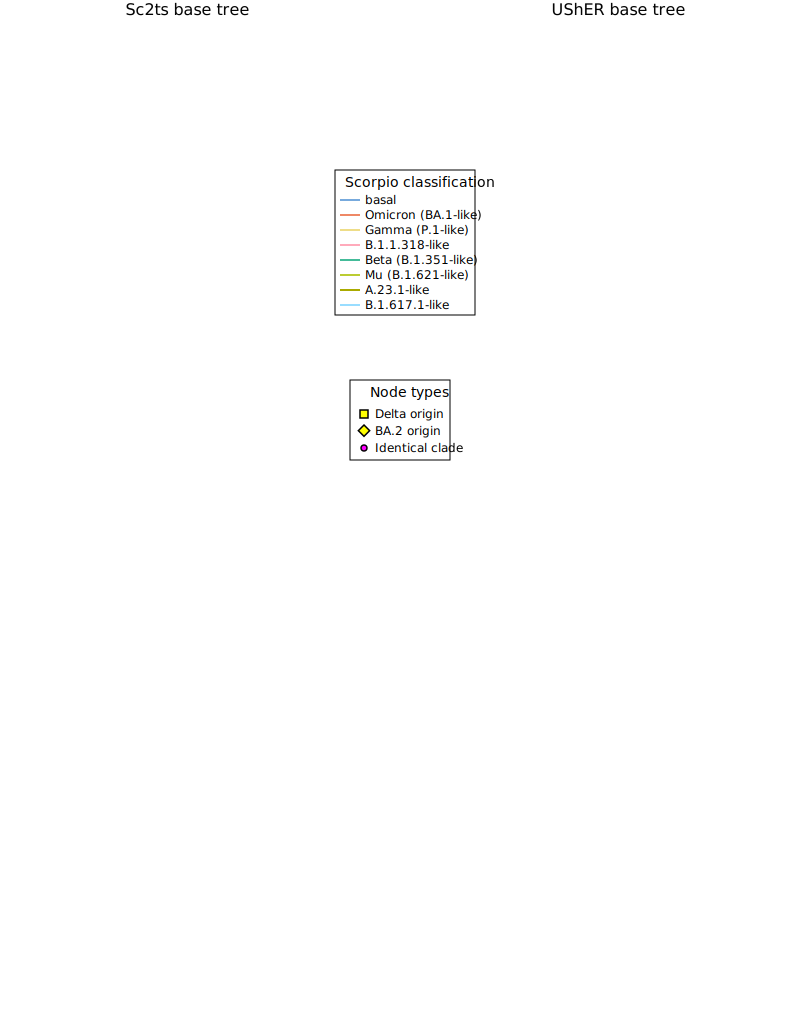
\includegraphics[width=\linewidth]{tanglegram_base_tree.pdf}
\caption{
Tanglegram comparing the basic phylogenetic backbones of sc2ts and UShER.
}
\label{fig:tanglegram_base}
\end{figure}

\begin{figure}
\centering
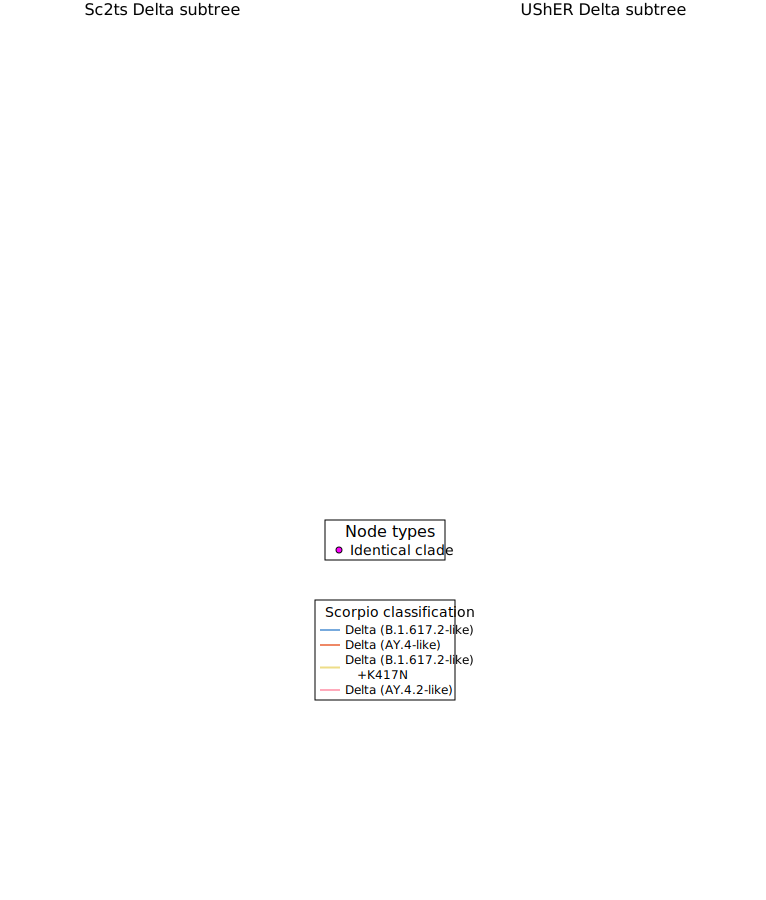
\includegraphics[width=\linewidth]{tanglegram_Delta_subtree.pdf}
\caption{
Tanglegram comparing sc2ts and UShER on the Delta subtree.
}
\label{fig:tanglegram_delta}
\end{figure}

\begin{figure}
\centering
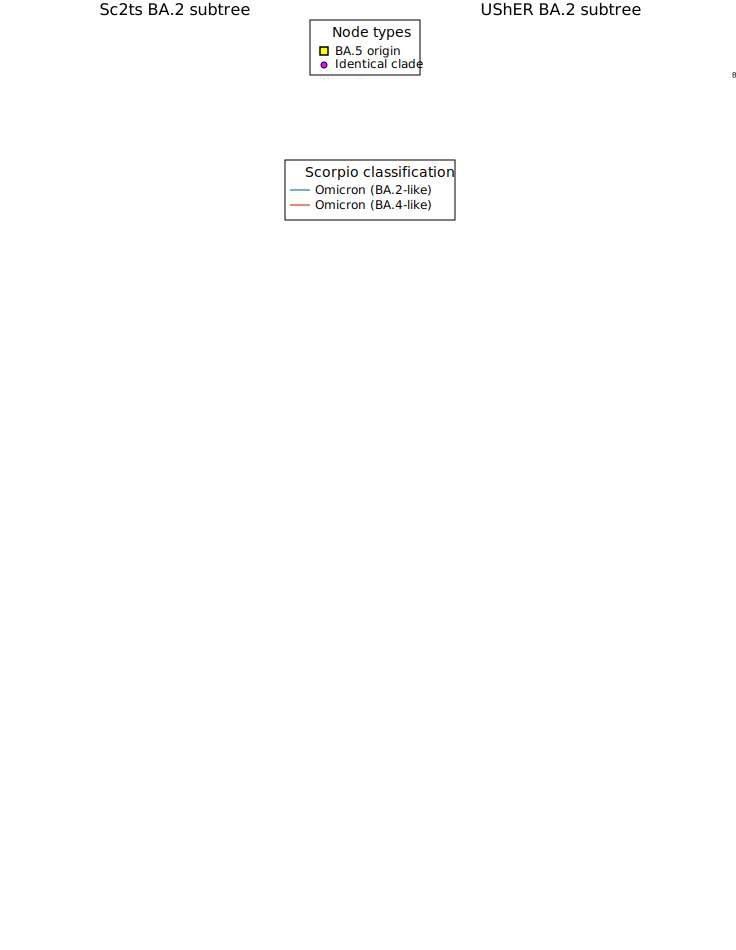
\includegraphics[width=\linewidth]{tanglegram_BA.2_subtree.pdf}
\caption{
Tanglegram comparing sc2ts and UShER on the BA.2 subtree.
}
\label{fig:tanglegram_ba2}
\end{figure}

\begin{figure}
\centering
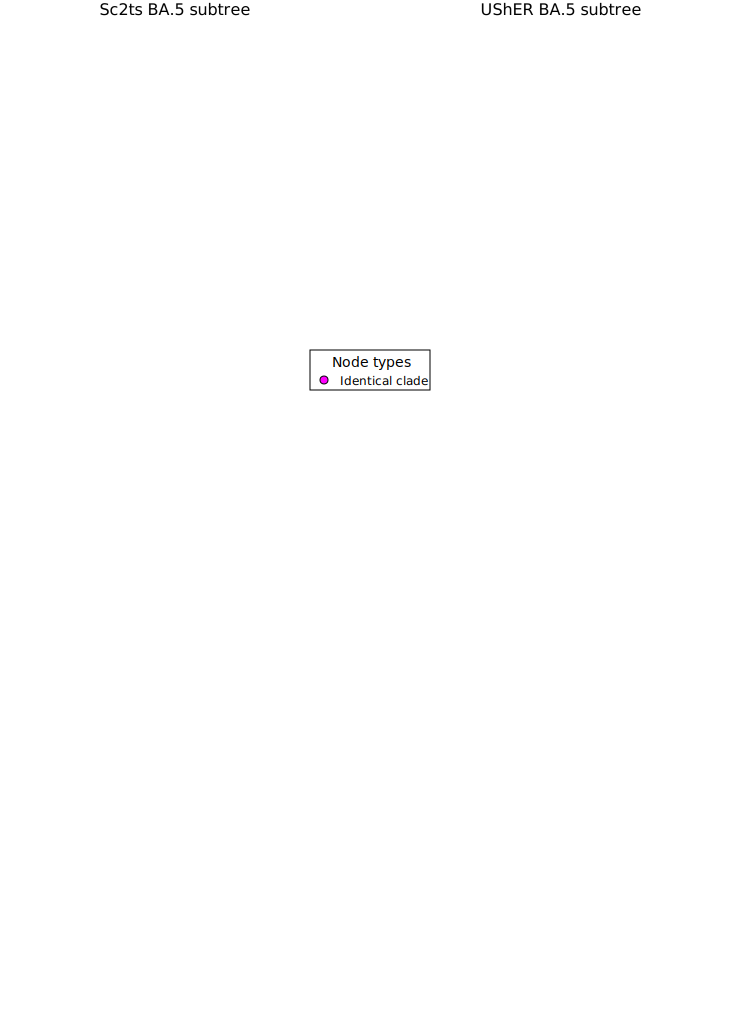
\includegraphics[width=\linewidth]{tanglegram_BA.5_subtree.pdf}
\caption{
Tanglegram comparing sc2ts and UShER on the BA.5 subtree.
}
\label{fig:tanglegram_ba5}
\end{figure}

\begin{figure}
\centering
\includegraphics[width=\linewidth]{mutational_spectra}
\caption{
All-site mutational spectra of major VOCs calculated from the sc2ts ARG (A),
the mutation count data from Bloom et al. (2023)\cite{Bloom2023} (B), and
the Viridian UShER phylogeny from Hunt et al. (2024)\cite{Hunt2024}.
}
\label{fig:mutational_spectra}
\end{figure}

\begin{figure}
\centering
\includegraphics[width=0.85\linewidth]{pango_vs_nextstrain_node_times.pdf}
\caption{
Inferred times of internal nodes corresponding to origins of Nextclade clades ($y$-axis) against those estimated in the Nextclade tree ($x$-axis). Confidence intervals shown as horizontal bars. Clades are labelled where dates differ by more than 28 days. 
}
\label{fig:pango_vs_nextstrain_node_times}
\end{figure}

\begin{figure}
\centering
\includegraphics[width=0.85\linewidth]{node_time_testing.pdf}
\caption{
Heat map showing differences (in days) between actual and re-estimated sample dates for a subset of internal sample nodes. 
}
\label{fig:node_time_testing}
\end{figure}

\begin{figure}
\centering
\includegraphics[width=0.85\linewidth]{subgraph-Alpha.pdf}
\caption{
Subgraph illustrating the saltational origin of B.1.1.7 (Alpha).
Squares represent sample nodes,
circles represent reconstructed internal nodes;
nodes classified as B.1.1.7 by Pangolin v4.3.1 are in pink.
Mutations are shown as rectangles along branches,
ordered by position; deletions are black.
Characteristic mutations
associated with the emergence of Alpha
are highlighted with a pink outline.
}
\label{fig:subgraph_alpha}
\end{figure}

\begin{figure}
\centering
\includegraphics[width=0.85\linewidth]{subgraph-Delta_recolored.pdf}
\caption{
Subgraph illustrating the origin of B.1.617.2 (Delta).
Symbols are described in \ref{fig:subgraph_alpha}, except that 
we highlight the characteristic mutations of Kappa and Delta:
those with a blue outline are listed
in the Pango designation issue \cite{PangoIssueKappa}
or the Kappa constellation \cite{ScorpioKappa},
but absent in the Delta constellation;
those with a purple outline are listed
in the Delta constellation \cite{ScorpioDelta}
or are Delta-specific deletions reported in Stern et al. \cite{Stern2021},
but absent in the Kappa constellation; and
those with a red outline are listed
in both the Kappa and Delta constellations.
We also outline
in orange the mutations associated with the lineage containing clades A to D and
in green those associated with lineage containing clade E.
Sites associated with multiple mutations in the subgraph
have their mutations assigned a unique fill colour
(orange, blue, green, red, etc);
reversions are further highlighted with a black outline.
Sc2ts seed samples (see Methods) for
B.1.617, B.1.617.1, and B.1.617.2 are plotted as red squares.
}
\label{fig:subgraph_delta}
\end{figure}

\begin{figure}
\centering
\includegraphics[width=0.85\linewidth]{subgraph-Omicron_recolored.pdf}
\caption{
Subgraph illustrating the saltational origin of
the major Omicron lineages BA.1 and BA.2.
Symbols are described in Figure~\ref{fig:subgraph_delta},
except that BA.1 samples are filled in light blue
(also used to outline BA.1 characteristic mutations),
BA.2 samples in light yellow
(also used to outline BA.2 characteristic mutations), and
B.1.1.529 mutations
which are neither BA.1 or BA.2 characteristic mutations are
outlined in green.
These colours correspond to those used
in the BA.1/BA.2 Pango designation issue \cite{RambautOmicron2021}.
}
\label{fig:subgraph_omicron}
\end{figure}

\newcommand{\cprheight}{1.5em}
% Add some more space between rows. Note this it would be sligntly nicer if the 
% label was aligned vertically in the center of the row, but this is good
% enough for now.
\renewcommand{\arraystretch}{2}

\begin{figure}
\centering
\begin{tabularx}{\textwidth}{>{\centering\arraybackslash}m{1cm}>{\arraybackslash}m{1cm}}
XC & \includegraphics[height=\cprheight]{static/XC.png}\\
XBR & \includegraphics[height=\cprheight]{static/XBR.png}\\
XA & \includegraphics[height=\cprheight]{static/XA.png}\\
XS & \includegraphics[height=\cprheight]{static/XS.png}\\
XL & \includegraphics[height=\cprheight]{static/XL.png}\\
XBG &\includegraphics[height=\cprheight]{static/XBG.png}\\
XQ & \includegraphics[height=\cprheight]{static/XQ++.png}\\
XBD & \includegraphics[height=\cprheight]{static/XBD.png}\\
XM & \includegraphics[height=\cprheight]{static/XM+XAL.png}\\
XBH & \includegraphics[height=\cprheight]{static/XBH.png}\\
XBB & \includegraphics[height=\cprheight]{static/XBB.png}\\
XY & \includegraphics[height=\cprheight]{static/XY.png}\\
XF & \includegraphics[height=\cprheight]{static/XF.png}\\
XBF & \includegraphics[height=\cprheight]{static/XBF.png}\\
XW & \includegraphics[height=\cprheight]{static/XW.png}\\
XG & \includegraphics[height=\cprheight]{static/XG.png}\\
\hline
Xx & \includegraphics[height=\cprheight]{static/XZ++.png}\\
XE/XH  & \includegraphics[height=\cprheight]{static/XE+XH.png}\\
XBM & \includegraphics[height=\cprheight]{static/XBM.png}\\
XJ & \includegraphics[height=\cprheight]{static/XJ.png}\\
XAF & \includegraphics[height=\cprheight]{static/XAF.png}\\
\end{tabularx}
\caption{Copying patterns for the 21 recombination events associated with Pango 
X lineages listed in Table~\ref{tab:pango_x_lineages} (in the same order). 
The horizontal line separates Type I and Type II events.
See also Document S3 for exact positions and nucleotide bases.}
\label{fig:pango_x_copying_patterns}
\end{figure}

% Reset this in case we make any more tables beyond this
\renewcommand{\arraystretch}{1}

\begin{figure}
\centering
\includegraphics[width=\linewidth]{recombinant_evidence_cov_recomb}
\caption{Properties of sc2ts recombination events, coloured by CovRecomb 
classification. All other details as per Figure~\ref{fig:recombinant_evidence}.
\label{fig:recombinant_evidence_cov_recomb}}
\end{figure}

\begin{figure}
\centering
\includegraphics[width=\linewidth]{recombinant_evidence_rebar}
\caption{Properties of sc2ts recombination events, coloured by rebar
classification. All other details as per Figure~\ref{fig:recombinant_evidence}.
\label{fig:recombinant_evidence_rebar}}
\end{figure}

% \begin{figure}
% \centering
% \includegraphics[width=\linewidth]{recombinant_evidence_ripples_p4}
% \caption{Things}
% \label{fig:recombinant_evidence_ripples_p4}
% \end{figure}

% \begin{figure}
% \centering
% \includegraphics[width=\linewidth]{recombinant_evidence_ripples_p3}
% \caption{Things}
% \label{fig:recombinant_evidence_ripples_p3}
% \end{figure}


\begin{figure}
\centering
\includegraphics[width=\linewidth]{recombinant_qc}
\caption{
Quality control of recombination events.
Scatterplot of recombination events by the net number of supporting loci
on the left parent (x-axis) and the right parent (y-axis).
The shaded regions highlight potentially artefactual recombination events,
which have fewer than 4 net supporting loci
on one side or both sides of the suggested breakpoint.
colours indicate the primer scheme used for sequencing.
The pie charts show breakdowns of the recombination events
by primer scheme per quadrant (labeled Q1 to Q4).
Recombination events associated with
the origins of Pango X and Jackson\cite{Jackson2021} lineages are labeled.
}
\label{fig:recombinant_qc}
\end{figure}

\renewcommand{\cprheight}{4.0em}

\begin{figure}
\centering
% NOTE the size of the second "m" column doesn't matter, but we have to fix the
% size in order for vertical centering to work :sigh:
% The layout here isn't ideal, but it's incredibly fiddly to get center
% alignment veritically with cells to work, so this is good enough.
\begin{tabularx}{0.85\textwidth}{>{\centering\arraybackslash}m{1cm}>{\arraybackslash}m{1cm}}
Q1 & \includegraphics[height=\cprheight]{static/RE_node-QCpass-427863.png}\\
Q2 & \includegraphics[height=\cprheight]{static/RE_node-QCfail-748991.png}\\
Q3 & \includegraphics[height=\cprheight]{static/RE_node-QCfail-411345.png}\\
Q4 & \includegraphics[height=\cprheight]{static/RE_node-QCfail-663484.png}\\
\end{tabularx}
\caption{
Illustrative copying patterns
drawn from the quadrants labelled in Figure~\ref{fig:recombinant_qc}. 
Each copying pattern shows the 
the positions
where the allelic state in a recombinant
(middle row, labelled by node ID)
matches that of the left (P0: upper row, coloured green) 
or right parent (P1: lower row, coloured blue),
or where the recombination event requires a de-novo mutation
(gold, with mutational change below).
Parental states that correspond to the reference but are not 
inherited by the recombinant are shown with a gray background.
Genome position (``pos'') and reference allele (``ref'') are
shown for each column.
Underneath the copying pattern, adjacent genomic positions are 
underlined in red, and
near-adjacent sites (within 3 bases) in orange.
}
\label{fig:copying_pattern_examples}
\end{figure}

\begin{figure}
\centering
\begin{tabular}{cc}
\includegraphics[width=0.5\linewidth]{ripples_p4_sc2ts_events.pdf}&
\includegraphics[width=0.5\linewidth]{ripples_p3_sc2ts_events.pdf}\\
(A) & (B) \\
\end{tabular}
\caption{Intersection of the RIPPLES and sc2ts recombination events at
different values of the RIPPLES parsimony parameter, p.}
\label{fig:ripples_sc2ts_events}
\end{figure}
 
\begin{figure} 
\centering
\includegraphics[width=0.5\textwidth]{LS_model_schematic}
\caption{
A schematic of the Li and Stephens (LS)
model, in which a focal sequence (bottom) is described as an
imperfect mosaic of the sequences in a reference panel.
Black crosses along the focal sequence show sequencing
errors or mutations.
In the standard formulation, at site $\ell$, the recombination probability is $r_\ell$,
the mutation probability is $\mu_\ell$ and $n$
denotes the size of the reference panel.
The Viterbi algorithm can be used to find a
``copying path'' through the reference panel for a given focal sequence that
maximises the likelihood under these parameters. Unseen states in the reference panel are shown as coloured lines enclosed by
the grey box. The black arrow describes the true path through the data which leads to the emitted
focal sequence below. Examples of transition and
emission probabilities along this trajectory are shown by the red and blue
arrows, respectively.
}
\label{fig:ls_diagram}
\end{figure}

\begin{figure}
\centering
\includegraphics[width=0.85\linewidth]{tree_ops}
\caption{
Parsimony improving heuristics. (A) Mutation collapsing. Mutation A100G is
shared by two siblings, and we create a new node to represent the ancestor
on which this mutation occurred. (B) Reversion pushing. Mutation A128C is
immediately reverted by C128A, and we create a new node to represent the 
ancestor that did not carry A128C.
}
\label{fig:parsimony_ops}
\end{figure}

%%%%%%%%%%%%%%%%
% Tables
%%%%%%%%%%%%%%%%

\clearpage
\section*{Supplementary Tables}

\begin{table}[h]
\centering
\caption{
Major deletion events in the ARG.
The deletions caused by these events
are inherited by at least 10,000 samples.
The deletions are characterized by
a site position in the genome (start) and
the number of sites involved (length);
they are annotated by the gene in which they occur
(non-coding otherwise).
The IDs of the nodes in the ARG
above which the deletions occur and
the Pango lineages assigned to these nodes are shown.
Frequency is the percentage of samples inheriting a deletion.
If a deletion has been identified
as a characteristic mutation of a VOC
by a study (or an analysis),
a reference to the study (or the analysis) is provided.
Abbreviations: NSP, non-structural protein;
ORF, open reading frame;
S, Spike;
S1-NTD, N-terminal domain in Spike S1 subunit.
}
\label{tab:major_dels}
\begin{tabular}{rccrcrrc}
\toprule
Start & Length & Region & Node & Pango lineage & Frequency (\%) & Ref\\
\midrule
28271 & 1 & non-coding & 1436808 & B.1 & 45.06 &  \\
28248 & 6 & ORF8 & 220186 & B.1.617.2 (Delta) & 44.91 & \cite{Stern2021} \\
22029 & 6 & S / S1-NTD & 200039 & B.1.617.2 (Delta) & 44.82 & \cite{Stern2021} \\
11288 & 4 & ORF1ab / NSP6 & 1436802 & B.1.1.529 (Omicron) & 35.12 &  \\
28362 & 9 & N & 1436802 & B.1.1.529 (Omicron) & 35.12 & \cite{RambautOmicron2021} \\
21633 & 9 & S / S1-NTD & 822854 & BA.2 (Omicron) & 21.44 & \cite{RambautOmicron2021} \\
11292 & 5 & ORF1ab / NSP6 & 822854 & BA.2 (Omicron) & 21.43 &  \\
6513 & 3 & ORF1ab / NSP3 & 851246 & BA.1 (Omicron) & 13.73 & \cite{RambautOmicron2021} \\
11283 & 5 & ORF1ab / NSP6 & 851246 & BA.1 (Omicron) & 13.69 &  \\
21765 & 6 & S / S1-NTD & 851246 & BA.1 (Omicron) & 13.68 & \cite{RambautOmicron2021} \\
21987 & 9 & S / S1-NTD & 851246 & BA.1 (Omicron) & 13.68 & \cite{RambautOmicron2021} \\
22194 & 3 & S / S1-NTD & 851246 & BA.1 (Omicron) & 12.60 & \cite{RambautOmicron2021} \\
28271 & 1 & non-coding & 86456 & B.1.1.7 (Alpha) & 11.70 &  \\
11288 & 9 & ORF1ab / NSP6 & 86456 & B.1.1.7 (Alpha) & 11.70 & \cite{RambautAlpha2020} \\
21991 & 3 & S / S1-NTD & 86456 & B.1.1.7 (Alpha) & 11.64 & \cite{RambautAlpha2020} \\
21765 & 6 & S / S1-NTD & 86456 & B.1.1.7 (Alpha) & 11.70 & \cite{RambautAlpha2020} \\
21765 & 6 & S / S1-NTD & 1265302 & BA.4 (Omicron) & 7.67 & \cite{Tegally2022} \\
686 & 9 & ORF1ab / NSP1 & 2698748 & BA.4 (Omicron) & 0.94 &  \\
\bottomrule
\end{tabular}
\end{table}


\begin{table}
\centering
\caption{
Recurrent deletions in the ARG.
These deletions occur on at least two branches in the ARG and
are found in the alignments of at least 10,000 (0.4\%) samples
in the Viridian v04 dataset.
For each deletion, the number of occurrences in the ARG and
the number of samples where it is observed are shown.
For further explanation,
see the caption of Table~\ref{tab:major_dels}.
Abbreviations:
NSP, non-structural protein;
ORF, open reading frame;
S, Spike;
S1-NTD, N-terminal domain in Spike S1 subunit.
}
\label{tab:rec_dels}
\begin{tabular}{rrcrr}
\toprule
Start & Length & Region & Occurrences & Samples\\
\midrule
686 & 9 & ORF1ab / NSP1 & 6436 & 43354\\
21991 & 3 & S / S1-NTD & 2088 & 309629\\
21765 & 6 & S / S1-NTD & 482 & 820194\\
22029 & 6 & S / S1-NTD & 275 & 1107941\\
22194 & 3 & S / S1-NTD & 200 & 310349\\
6513 & 3 & ORF1ab / NSP3 & 181 & 341380\\
21987 & 9 & S / S1-NTD & 70 & 338633\\
28248 & 6 & ORF8 & 28 & 1113392\\
28271 & 1 & non-coding & 24 & 1331409\\
11288 & 9 & ORF1ab / NSP6 & 19 & 843291\\
11283 & 9 & ORF1ab / NSP6 & 13 & 339810\\
28362 & 9 & N & 7 & 850483\\
21633 & 9 & S / S1-NTD & 7 & 531973\\
\bottomrule
\end{tabular}
\end{table}


\begin{table}
\caption{
Concordance among methods in characterizing Pango X lineages.
These comparisons focus on the Pango X lineages associated with
the Type 1 recombination events (Table~\ref{tab:pango_x_lineages})
For each method, we calculated the number of Pango X lineages
which have inferred parent Pango lineages and breakpoint intervals
concordant with those proposed by the community.
The denominators indicate the number of Pango X lineages
for which detection results are available from the original
studies\cite{Alfonsi2024,Li2024CovRecomb}.
For the Pango X lineages with non-overlapping breakpoint intervals,
the distances between the inferred breakpoint intervals and
those proposed by the community are shown (median and range).
}
\label{tab:method_concordance}
\centering
\begin{tabular}{lccl}
\toprule & \multicolumn{1}{c}{Parent lineages} & \multicolumn{2}{c}{Breakpoint intervals} \\
\cmidrule(lr){2-2} \cmidrule(lr){3-4}
Method & Concordant (\%) & Concordant (\%) & Distance (bases) \\
\midrule
Sc2ts & 14 / 16 (87.5) & 14 / 16 (87.5) & 540.5 (315, 766)\\
RecombinHunt-GISAID & 13 / 15 (86.7) & 10 / 15 (66.7) & 764.0 (4, 1202)\\
RecombinHunt-Nextstrain & 12 / 15 (80.0) & 11 / 15 (73.3) & 1160.0 (559, 2785)\\
CovRecomb & 7 / 8 (87.5) & 4 / 8 (50.0) & 1562.5 (217, 13208)\\
\bottomrule
\end{tabular}
\end{table}

\begin{table}
\centering
\caption{
Sc2ts detection results for Pango X lineages not added to the ARG.
The number of samples in Viridian v04 dataset
assigned to these Pango X lineages,
the number of samples that passed sequence-level quality control, and
the number of recombination breakpoints
in the Viterbi solutions of the samples
are shown.
}
\label{tab:extra_hmm_results}
\begin{tabular}{crrr}
\toprule
Pango & Samples in Viridian & Samples passing QC & Breakpoints \\
\midrule
XBJ & 2 & 1 & 1\\
XBP & 8 & 2 & 1\\
XBS & 19 & 15 & 1\\
XBW & 1 & 1 & 1\\
XCA & 11 & 4 & 1\\
XAK & 2 & 2 & 1\\   % Multiple breakpoint Pango X
XAY & 15 & 11 & 6\\ % Multiple breakpoint Pango X
XBC & 36 & 21 & 3\\ % Multiple breakpoint Pango X
XBL & 2 & 2 & 0\\   % Multiple breakpoint Pango X
XBT & 1 & 1 & 2\\   % Multiple breakpoint Pango X
\bottomrule
\end{tabular}
\end{table}

% 2 + 8 + 19+ 1 + 11+ 2 + 15+ 36+ 2 + 1
% 97



\begin{table}
\caption{Validation of sc2ts recombinants by 3SEQ, CovRecomb and rebar over 
all 855 recombinants and the 354 passing and 501 failing QC.
}
\label{tab:recombinant_validation}
\centering
\begin{tabular}{llll}
\toprule
Method & Total    & QC Pass & QC Fail \\
\midrule
3SEQ        & 484 & 338     & 146 \\
CovRecomb   & 92  & 90      & 2\\
rebar       & 213 & 203     & 10 \\
\bottomrule
\end{tabular}
\end{table}



\begin{table}
\caption{
RIPPLES events associated with Pango X lineages.
Each row is a recombination event identified by RIPPLEs (at $p=3$)
in which Pango X lineages appear,
along with the corresponding sc2ts event from Table~\ref{tab:pango_x_lineages},
where applicable, grouped by class.
Events also present at $p=4$ are indicated.
Clades are matched by finding the most recent common ancestor of
the samples associated with each UShER+RIPPLES event in the sc2ts ARG.
The clade differences indicates the closeness of the match.
}
\label{tab:ripples_x_lineages}
\centering
\begin{scriptsize}

\begin{tabular}{lrrlrl}
\toprule
sc2ts event & in $p=4$ & UShER desc & sc2ts class & clade diff & descendants \\
\midrule
\multicolumn{6}{l}{Equivalent Sc2ts and RIPPLES recombination events}\\
XC & $\checkmark$ & 5 & I & 0 & {XC:5} \\
XBR & $\checkmark$ & 1 & I & 0 & {XBR:1} \\
% XM3 & $\checkmark$ & 1 & I & 0 & {XM:1} \\
XS & $\checkmark$ & 17 & I & 0 & {XS:17} \\
XA & $\checkmark$ & 39 & I & 0 & {XA:39} \\
XY &  & 23 & I & 0 & {XY:23} \\
XW &  & 32 & I & 0 & {XW:32} \\
XL &  & 64 & I & 0 & {XL:64} \\
XBB &  & 6452 & I & 1 & {XBB:6452} \\
\midrule
\multicolumn{6}{l}{RIPPLEs recombination event close to sc2ts recombination event}\\
XBM & $\checkmark$ & 12 & II & 0 & {XBM:10, BF.3:2} \\
XM & $\checkmark$ & 8 & II & 0 & {XM:4, BA.2:4} \\
Xx & $\checkmark$ & 18 & II & 0 & {XAC:18} \\
Xx &  & 9 & II & 0 & {XAE:9} \\
XQ &  & 1 & II & 0 & {XAM:1} \\
XQ &  & 21 & II & 0 & {XAM:21} \\
XE/XH &  & 1113 & II & 3 & {XE:1113} \\
\midrule
\multicolumn{6}{l}{RIPPLEs recombination event equivalant to sc2ts non-recombination event}\\
XB & $\checkmark$ & 411 & IV & 0 & {XB:192, B.1:219} \\
\midrule
\multicolumn{6}{l}{RIPPLEs recombination event not comparable to sc2ts}\\
NA & $\checkmark$ & 19 & NA & 45190 & {XAJ:18, BA.4:1} \\
NA & $\checkmark$ & 35 & NA & 7147 & {XBD:30, BA.2.75:5} \\
NA & $\checkmark$ & 36 & NA & 7146 & {XBR:1, XBD:30, BA.2.75:5} \\
NA &  & 20 & NA & 1061775 & {XS:17, BA.1:1, BA.1.1:1, BA.1.15:1} \\
NA &  & 1321 & NA & 340501 & {XE:1113, XJ:68, BA.2:82, XM:29, XY:23,
XAL:3, XAF:1, XH:2} \\
\bottomrule
\end{tabular}

\end{scriptsize}
\end{table}

\begin{table}
\centering
\caption{
Comparison of recombination breakpoint
intervals and parent lineages for Groups A-D
reported by Jackson et al.\ with the corresponding
recombination events in the sc2ts ARG.
The second column gives the number of sequences in the group.
See the text for details of the groups and the sequences included.
limited to the samples considered by Jackson et al.
The breakpoint coordinates in Table 1 of Jackson et al.\ have been altered as follows: 
we subtract one to the left coordinates and add one to the right coordinates 
to correspond to the \texttt{tskit} definition of inheritance on either side of a breakpoint,
and add one to the right coordinate to make the intervals right-exclusive.
}
\label{tab:jackson}
\begin{tabular}{lllr@{--}lr@{+}l}
\toprule
Group & Sequences & Method & \multicolumn{2}{c}{Breakpoint interval} & \multicolumn{2}{r}{Parent lineages} \\
\midrule
A (XA)       & 2   & Jackson        &  21,254&21,767 & B.1.177&B.1.1.7 \\
             &     &\texttt{sc2ts} &  20,411&21,765 & B.1.177.18&B.1.1.7 \\
\cmidrule{3-7}
B            & 2   & Jackson        &  6,527&6,956 & B.1.36.28&B.1.1.7  \\
             &     &\texttt{sc2ts} &   6,529&6,954 & B.1.36.28&B.1.1.7  \\
\cmidrule{3-7}
C            & 3   &Jackson         &  24,913&28,653 &  B.1.1.7&B.1.221 \\
             &     &\texttt{sc2ts} &  25,997&27,972 &  B.1.1.7&B.1.221.1 \\
\cmidrule{3-7}
D            & 3   & Jackson        &  21,574&23,065 &  B.1.36.17&B.1.1.7 \\
             &     &\texttt{sc2ts} &  22,445&23,063 &  B.1.36.39&B.1.1.7 \\
\bottomrule
\end{tabular}
\end{table}


\begin{table}
\caption{
Distribution of numbers of descendants for UShER+RIPPLES events
and sc2ts. The first column shows the number of descendants (binned
for larger values) and the others show the corresponding number of events.
}
\label{tab:ripples_sc2ts_event_descendants}
\centering
\begin{tabular}{lrrr}
\toprule
Count & RIPPLES p3 & RIPPLES p4 & sc2ts \\
\midrule
1 & 2616 & 757 & 525 \\
2 & 575 & 178 & 124 \\
3 & 232 & 65 & 47 \\
4 & 124 & 38 & 32 \\
5 & 74 & 14 & 17 \\
5-100 & 437 & 108 & 96 \\
100-1000 & 32 & 6 & 8 \\
1000-10k & 15 & 6 & 4 \\
10k-100k & 2 & 0 & 0 \\
100k-1m & 4 & 2 & 2 \\
\bottomrule
\end{tabular}
\end{table}



\end{document}
